\chapter{Implementation}
\label{chap:implementation}
\begin{chapterabstract}
The~implementation of the~EyeTrackingUtilities plug-in is described in this chapter. When added to an~Unreal Engine project, it offers a~Blueprint and Material directory in its Content folder. The~project can immediately use its contents.
\end{chapterabstract}

\section{Materials}

Materials are key to the~functionality of visualisation and collection of heatmaps. All of them will be described in this section. Material Content folder can be seen in Figure~\ref{fig:material-folder}.

\begin{figure}[!ht]\centering
    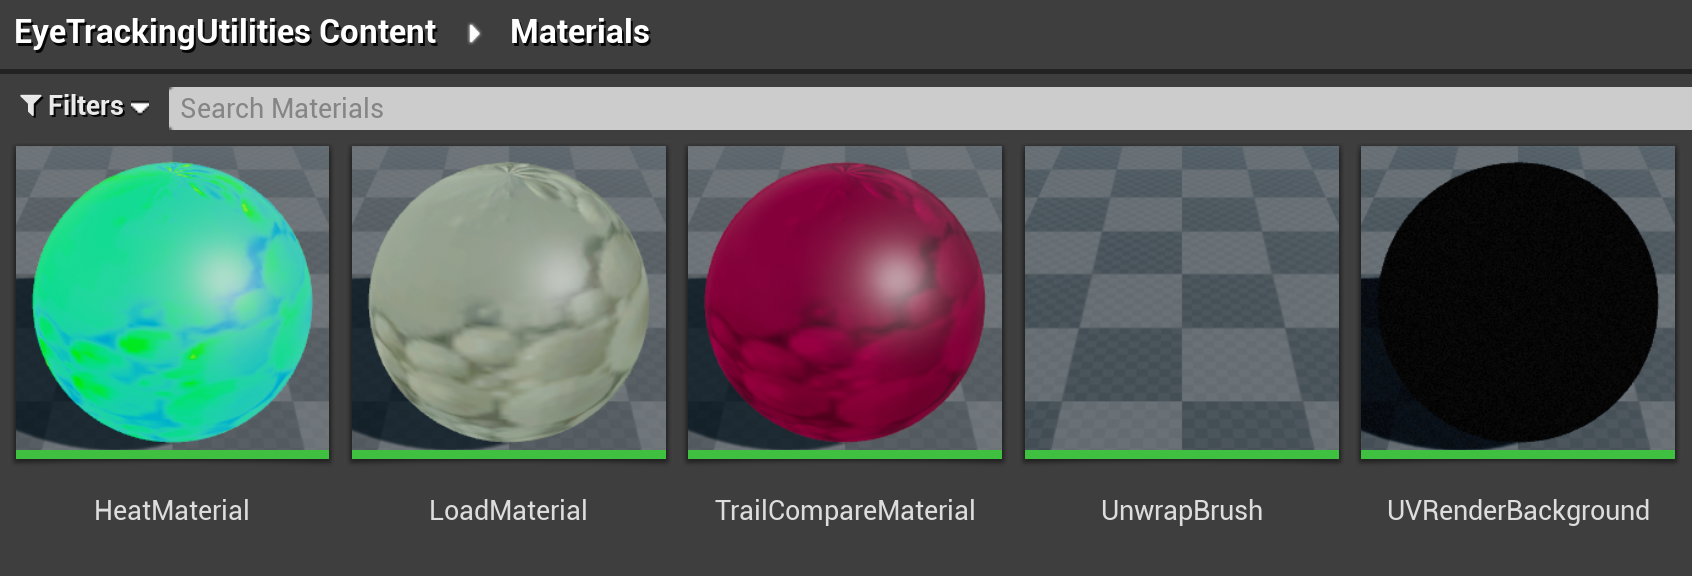
\includegraphics[width=\textwidth]{img/plugin-materials.png}
    \caption{Contents of EyeTrackingUtilities Material folder.}
    \label{fig:material-folder}
\end{figure}

\subsection{LoadMaterial and UVRenderBackground}
These are the~two simplest materials. \emph{UVRenderBackground} is a~material that constantly assigns a~black colour -- a~value of (0, 0, 0) -- to the~base colour, metallic, and specular pins of its result node.

\emph{LoadMaterial} is exactly the~same Material described in Section~\ref{sec:texture-loading}, to load already exported heatmap textures.
\pagebreak{}

\subsection{UnwrapBrush}
\label{sec:unwrap-brush-implementation}

\emph{UnwrapBrush} is an~implemented version of the~Material from Section~\ref{sec:uv-unwrap-method} using Tran's modification to skip several rendering steps using a~3D brush. The~block of material expressions in Figure~\ref{fig:unwrap-offset} is connected to the~World Position Offset pin of the~resulting Material node, and another part in Figure~\ref{fig:unwrap-3d-brush} is connected to Emissive Colour pin.

This technique enables rendering heatmap textures on a~GPU, so the~computation is very fast and does not slow down the~overall performance even when rendering 2K textures. However, it does have one problem, which is related to the~use of a~3D brush. If the~brush is large enough or even larger than the~object itself, it paints the~parts of the~object that are not visible. An~illustrative video demonstration is available in the~enclosed media in \path{video/02-3D-brush-problem.mp4}.

This problem was solved by adding two parameters related to a~collision in the~scene. The~solution can be seen in Figure 4.2.

\subsubsection*{HitNormal parameter}
\emph{HitNormal} is the~normal of the~static mesh at the~collision point in world coordinates. The~reason to use this is so that one can determine which pixel to colour based on the~size of an~angle between the~normal of a~currently drawn pixel in world coordinates and the~normal of the~collision point. This is to prevent the~brush from drawing on faces with an~opposite normal; those that are at an~obtuse angle to the~collision point.

When this angle is greater than $92{^\circ}$, the~pixel is assigned a~black colour. A~$90{^\circ}$ could have been used, but that would have prohibited the~simultaneous drawing on two perpendicular faces, which is desirable in some situations because both faces can be viewed at $45{^\circ}$.

But that does not solve the~whole problem because it is calculated only from the~object's perspective. It is still possible to draw on surfaces perpendicular to those on which the~collisions occur, even though they are not visible from the~camera view. 

\subsubsection*{DirectionToCamera parameter}
The~\emph{DirectionToCamera} parameter handles just that. The~method is exactly the~same as for the~previous parameter, but a~different threshold is set. It takes a~direction vector to the~camera and a~normal of the~pixel in the~WS. It will draw on all surfaces as long as the~camera is looking at them at $88{^\circ}$.

Note that using both of these angular conditions simultaneously will sometimes not guarantee drawing on a~face that is visible but not colliding with a~ray. The~former condition will guarantee that one can draw only on one of the~two faces that form an~acute-angle edge. At the~same time, however, it is not enough to use only the~latter condition, because sometimes the~brush may bleed through to the~other side of narrow objects and acute angles of the~camera.

\subsection{HeatMaterial}
\label{sec:heat-material-implementation}

Basic Material that visualises a~heatmap texture on a~mesh. Composed of four colours that are interpolated by the~value of one texture channel, as shown in Figure~\ref{fig:heatmap-material}~\cite{basic-heatmap-tutorial}. The~result is projected as the~colour of the~mesh. A~heatmap texture is added using the~texture parameter \emph{HeatTrail}. 

\pagebreak{}

\begin{figure}[!htb]\centering
    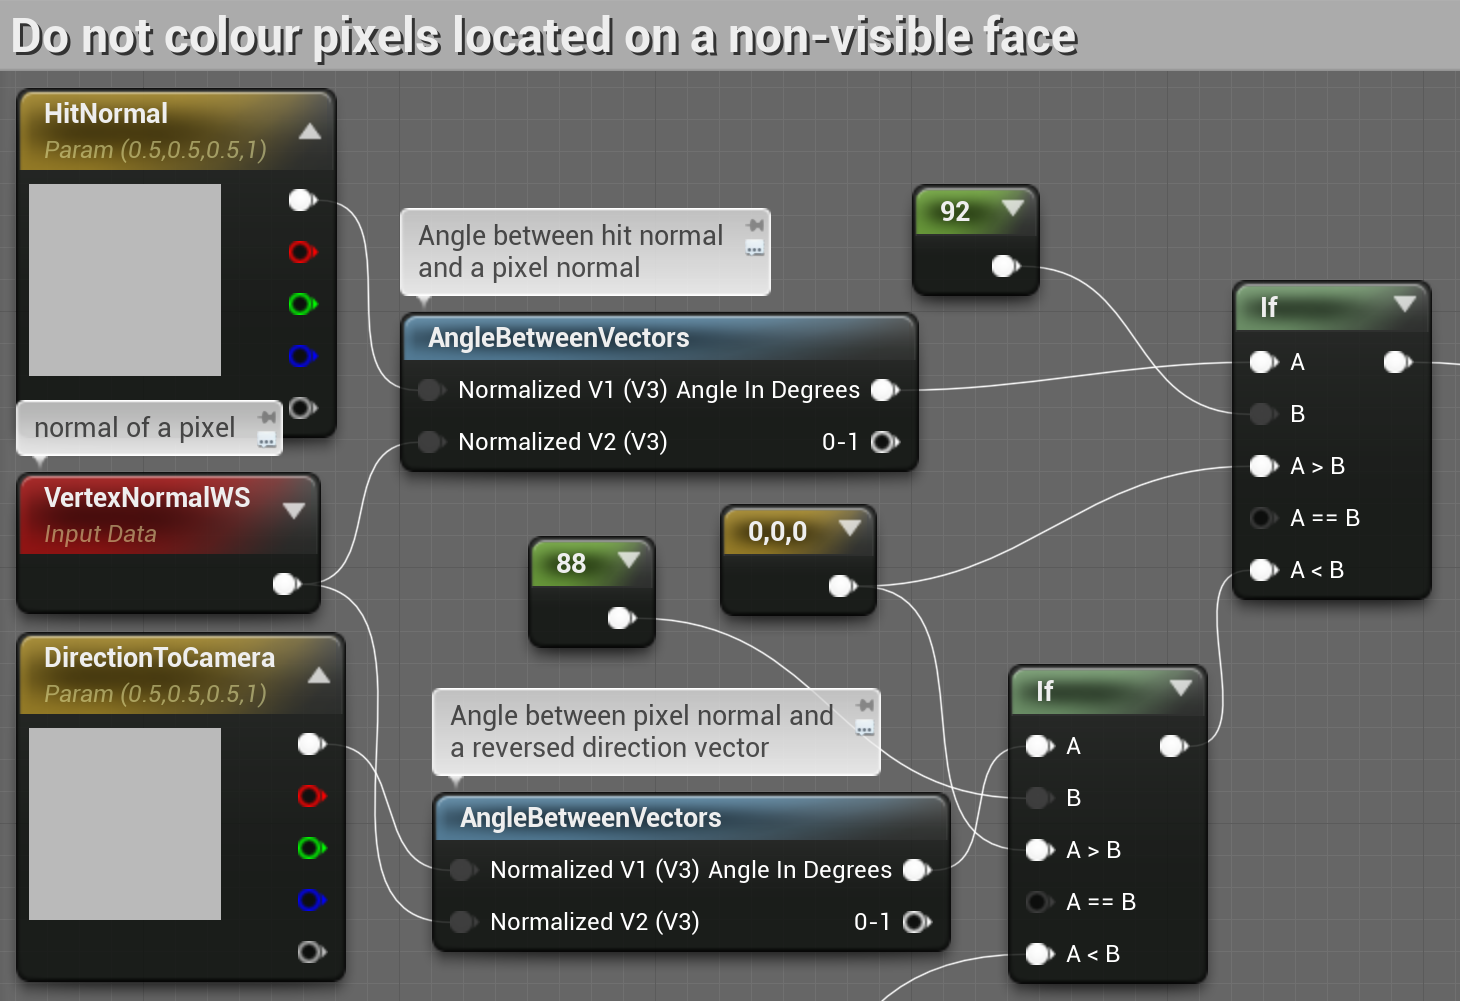
\includegraphics[width=\textwidth]{img/unwrap-brush-correction.png}
    \caption{Unwrap 3D brush material correction with angular conditions.}
    \label{fig:unwrap-brush-correction}
\end{figure}

\begin{figure}[!htb]\centering
    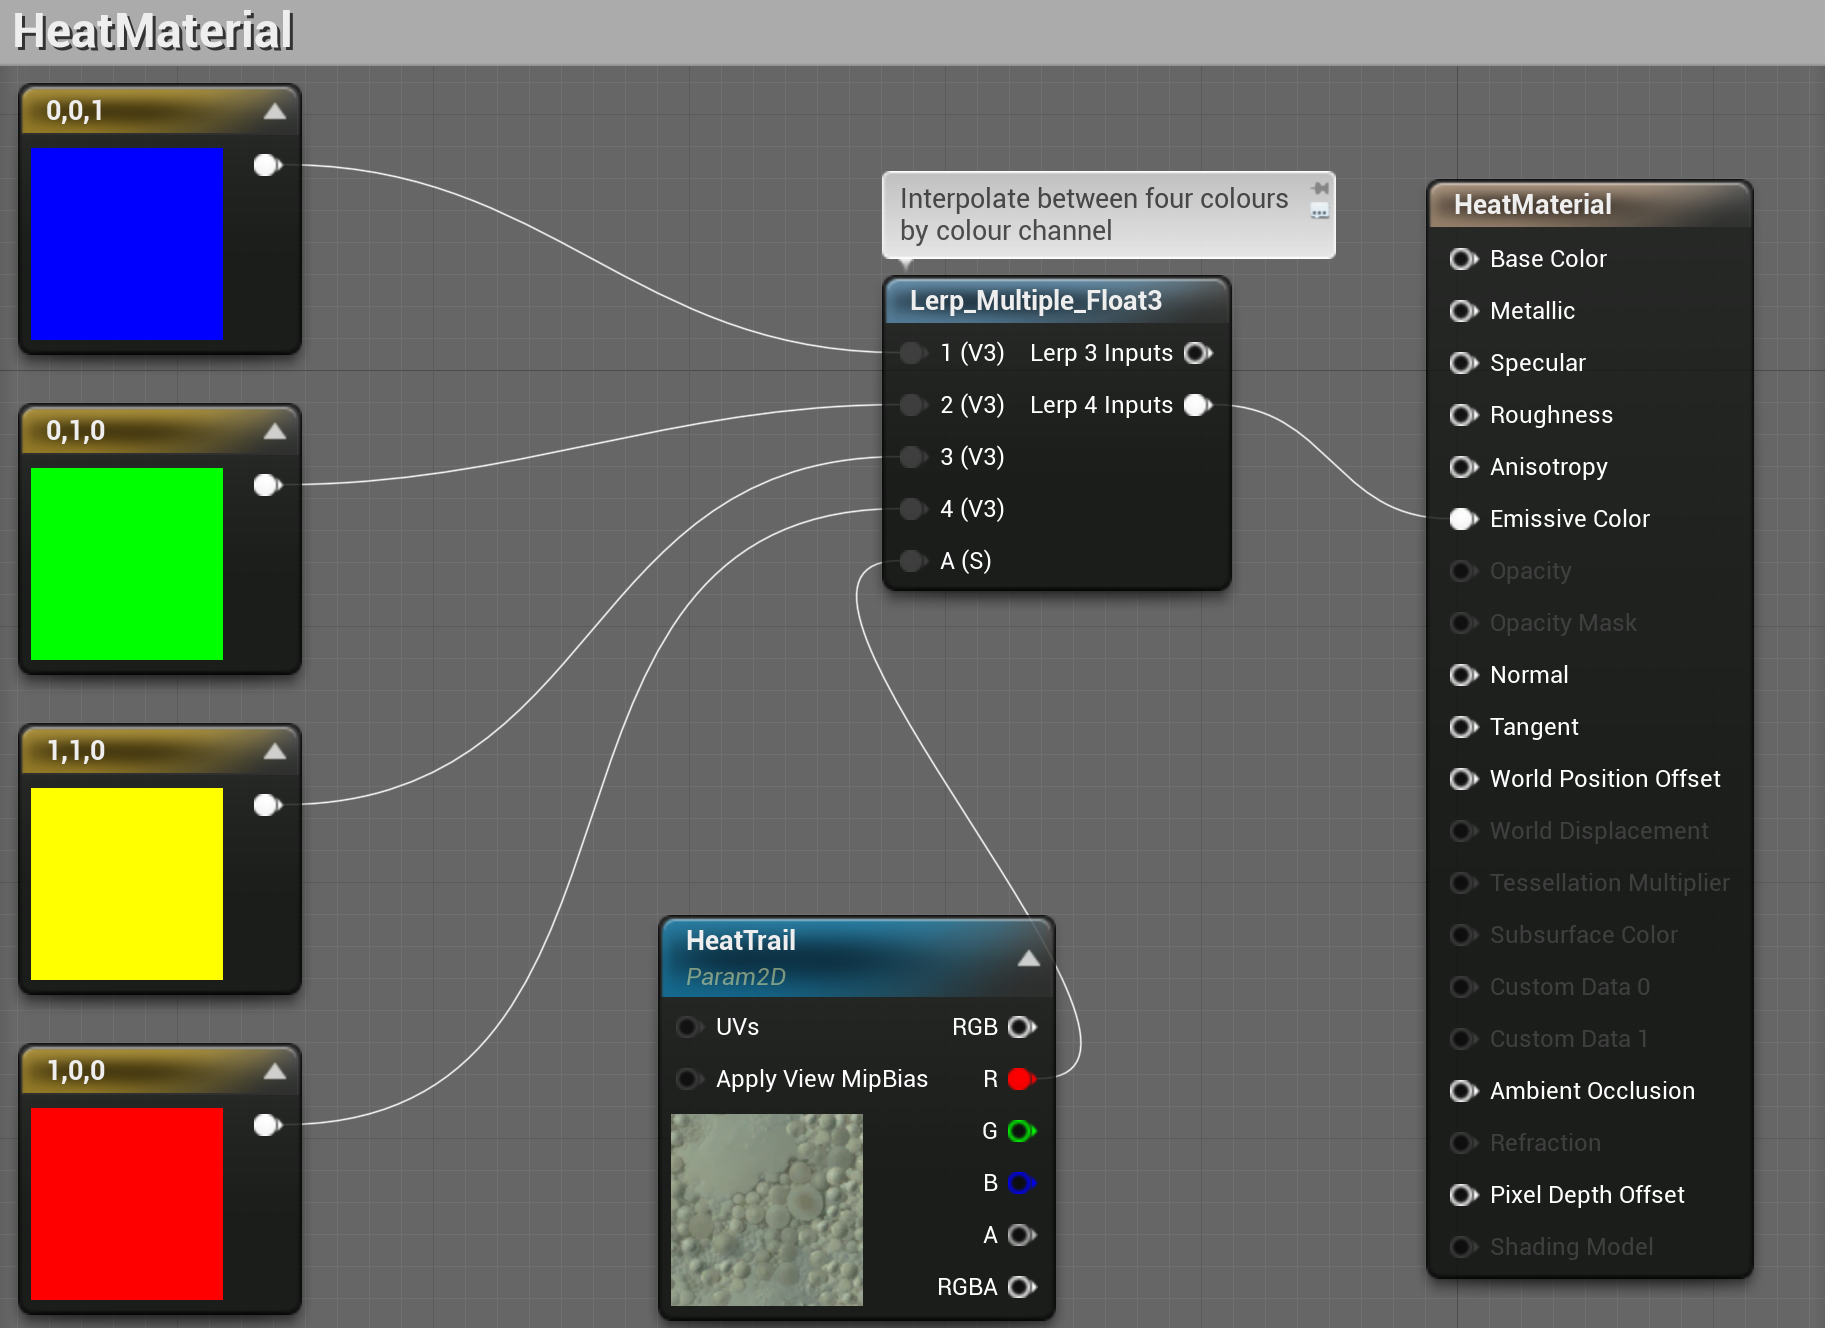
\includegraphics[width=0.85\textwidth]{img/heat-material.png}
    \caption{HeatMaterial node definition.}
    \label{fig:heatmap-material}
\end{figure}


\subsection{TrailCompareMaterial}
\label{sec:trail-compare-implementation}

Simple material that combines two colours into one to visualise the~appearance of two different textures on an~object with a~heatmap. The~definition is described in Figure~\ref{fig:trail-compare}.

\begin{figure}[!ht]\centering
    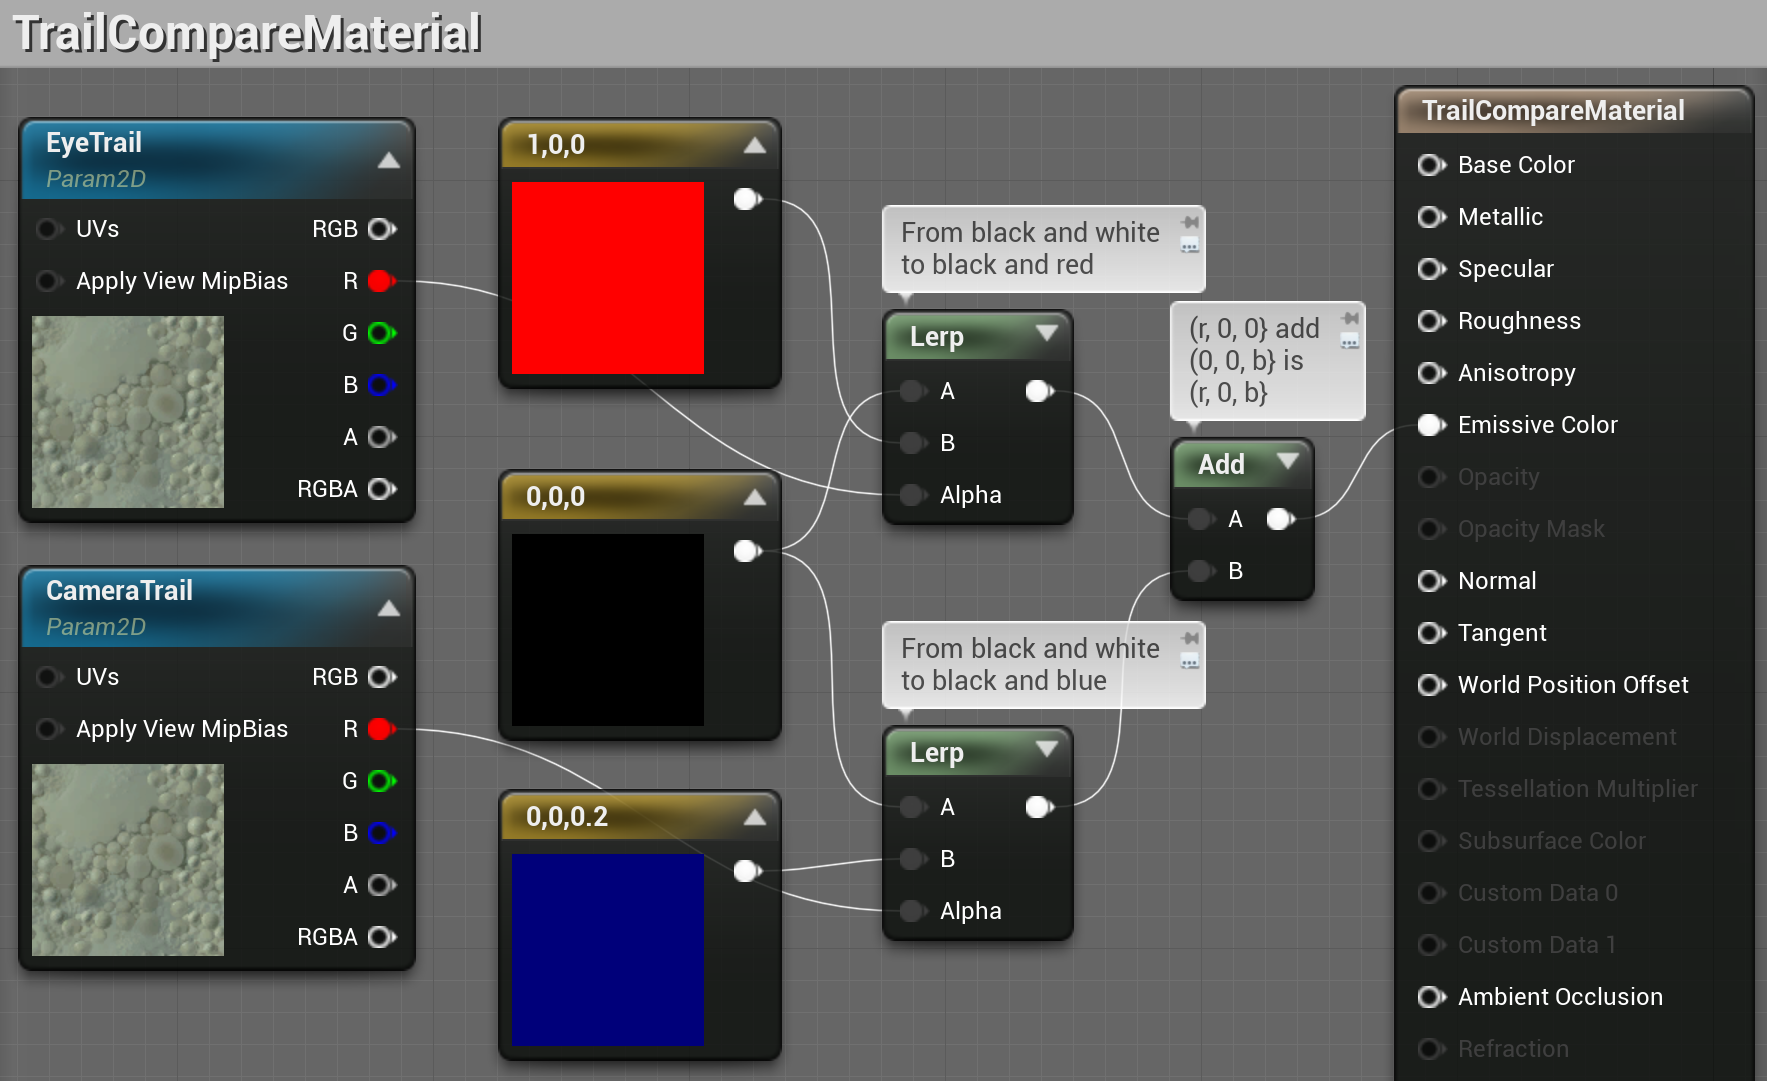
\includegraphics[width=\textwidth]{img/trail-compare-material.png}
    \caption{TrailCompareMaterial node definition.}
    \label{fig:trail-compare}
\end{figure}

\section{Blueprints}

This section presents the~implementation of classes with functionalities designed in Section~\ref{sec:plugin-functionality}. Contents of the~plug-in's Blueprint folder is in Figure~\ref{fig:blueprint-folder} 

\begin{figure}[!ht]\centering
    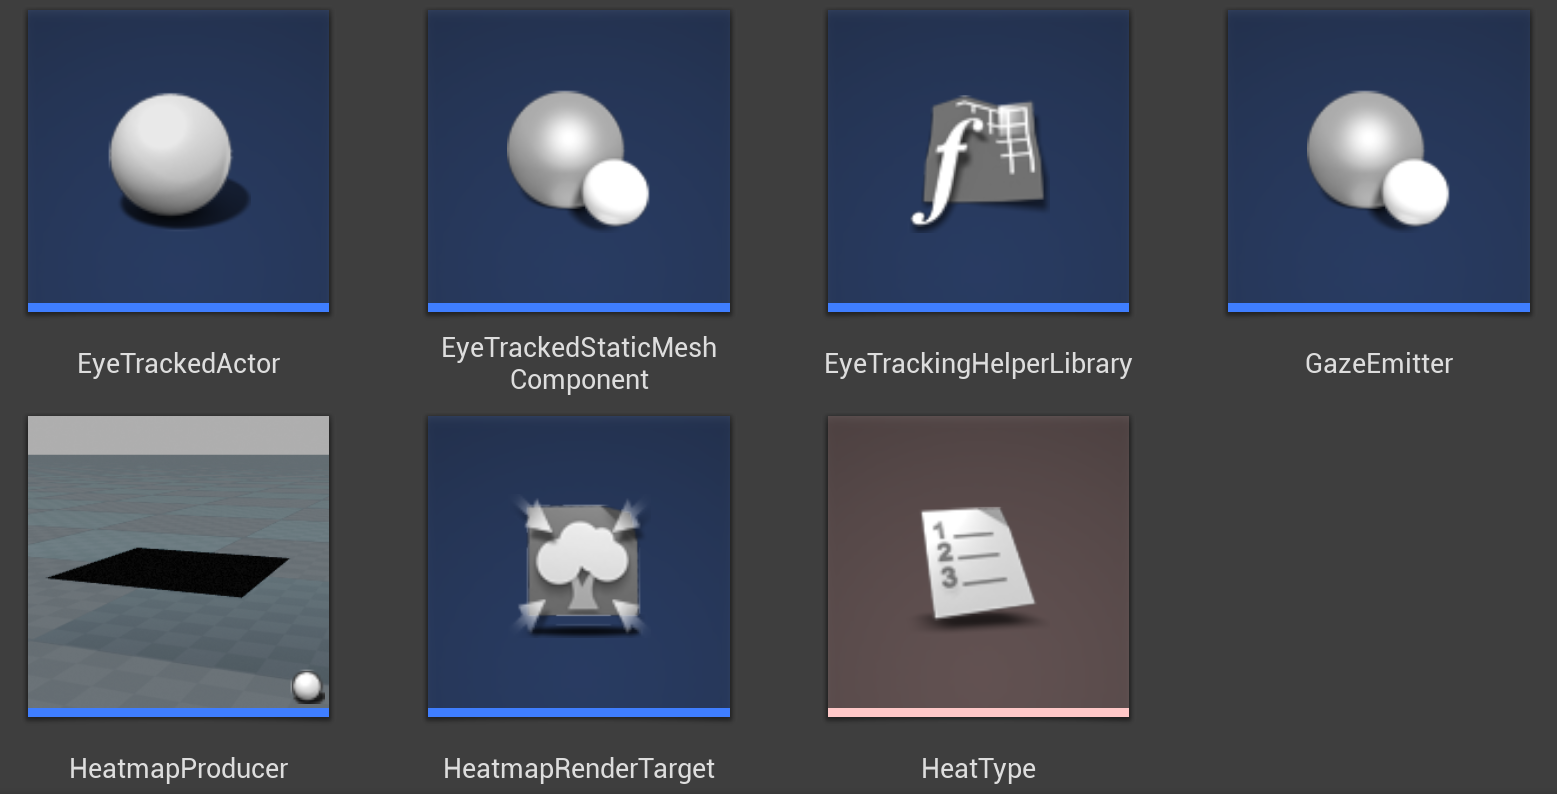
\includegraphics[width=0.8\textwidth]{img/plugin-blueprints.png}
    \caption{Contents of EyeTrackingUtilities Blueprint folder.}
    \label{fig:blueprint-folder}
\end{figure}

\subsection{EyeTrackedStaticMeshComponent}
\label{sec:static-mesh-ET}

\emph{EyeTrackedStaticComponent} is a~component inherited from \emph{StaticMeshComponent}. This class extends the~original static mesh functionality with two private render targets; \emph{EyeTrailTexture}, \emph{CameraTrailTexture}; and two private material instances; \emph{HeatmapMaterial}, \emph{CompareTrailMaterial}.

Both render targets have an~adjustable resolution in one variable that is initiated once when the~application starts. One is enough, because the~render targets must be a~square. Furthermore, it can be decided that a~given component can be EyeTracked but does not have to have its own heatmap, so a~public boolean \emph{AcceptsHeat} property was added.

The~render target is initialised by calling a~single Blueprint function called Create Canvas Render Target 2D, which is given a~width and height. This is done twice in total, as illustrated in Figure~\ref{fig:RT-init}. Furthermore, both instances of dynamic materials are initialised. Blueprint nodes of this operation can be seen in Appendix~\ref{appendix:ETcomponent}.

Render targets are private variables. To use them for rendering, a~Scene Capture Component from other classes will have targets assigned within this class. The~function \emph{AttachRenderer} in Figure~\ref{fig:attach-renderer} serves this purpouse.

\begin{figure}[!ht]\centering
    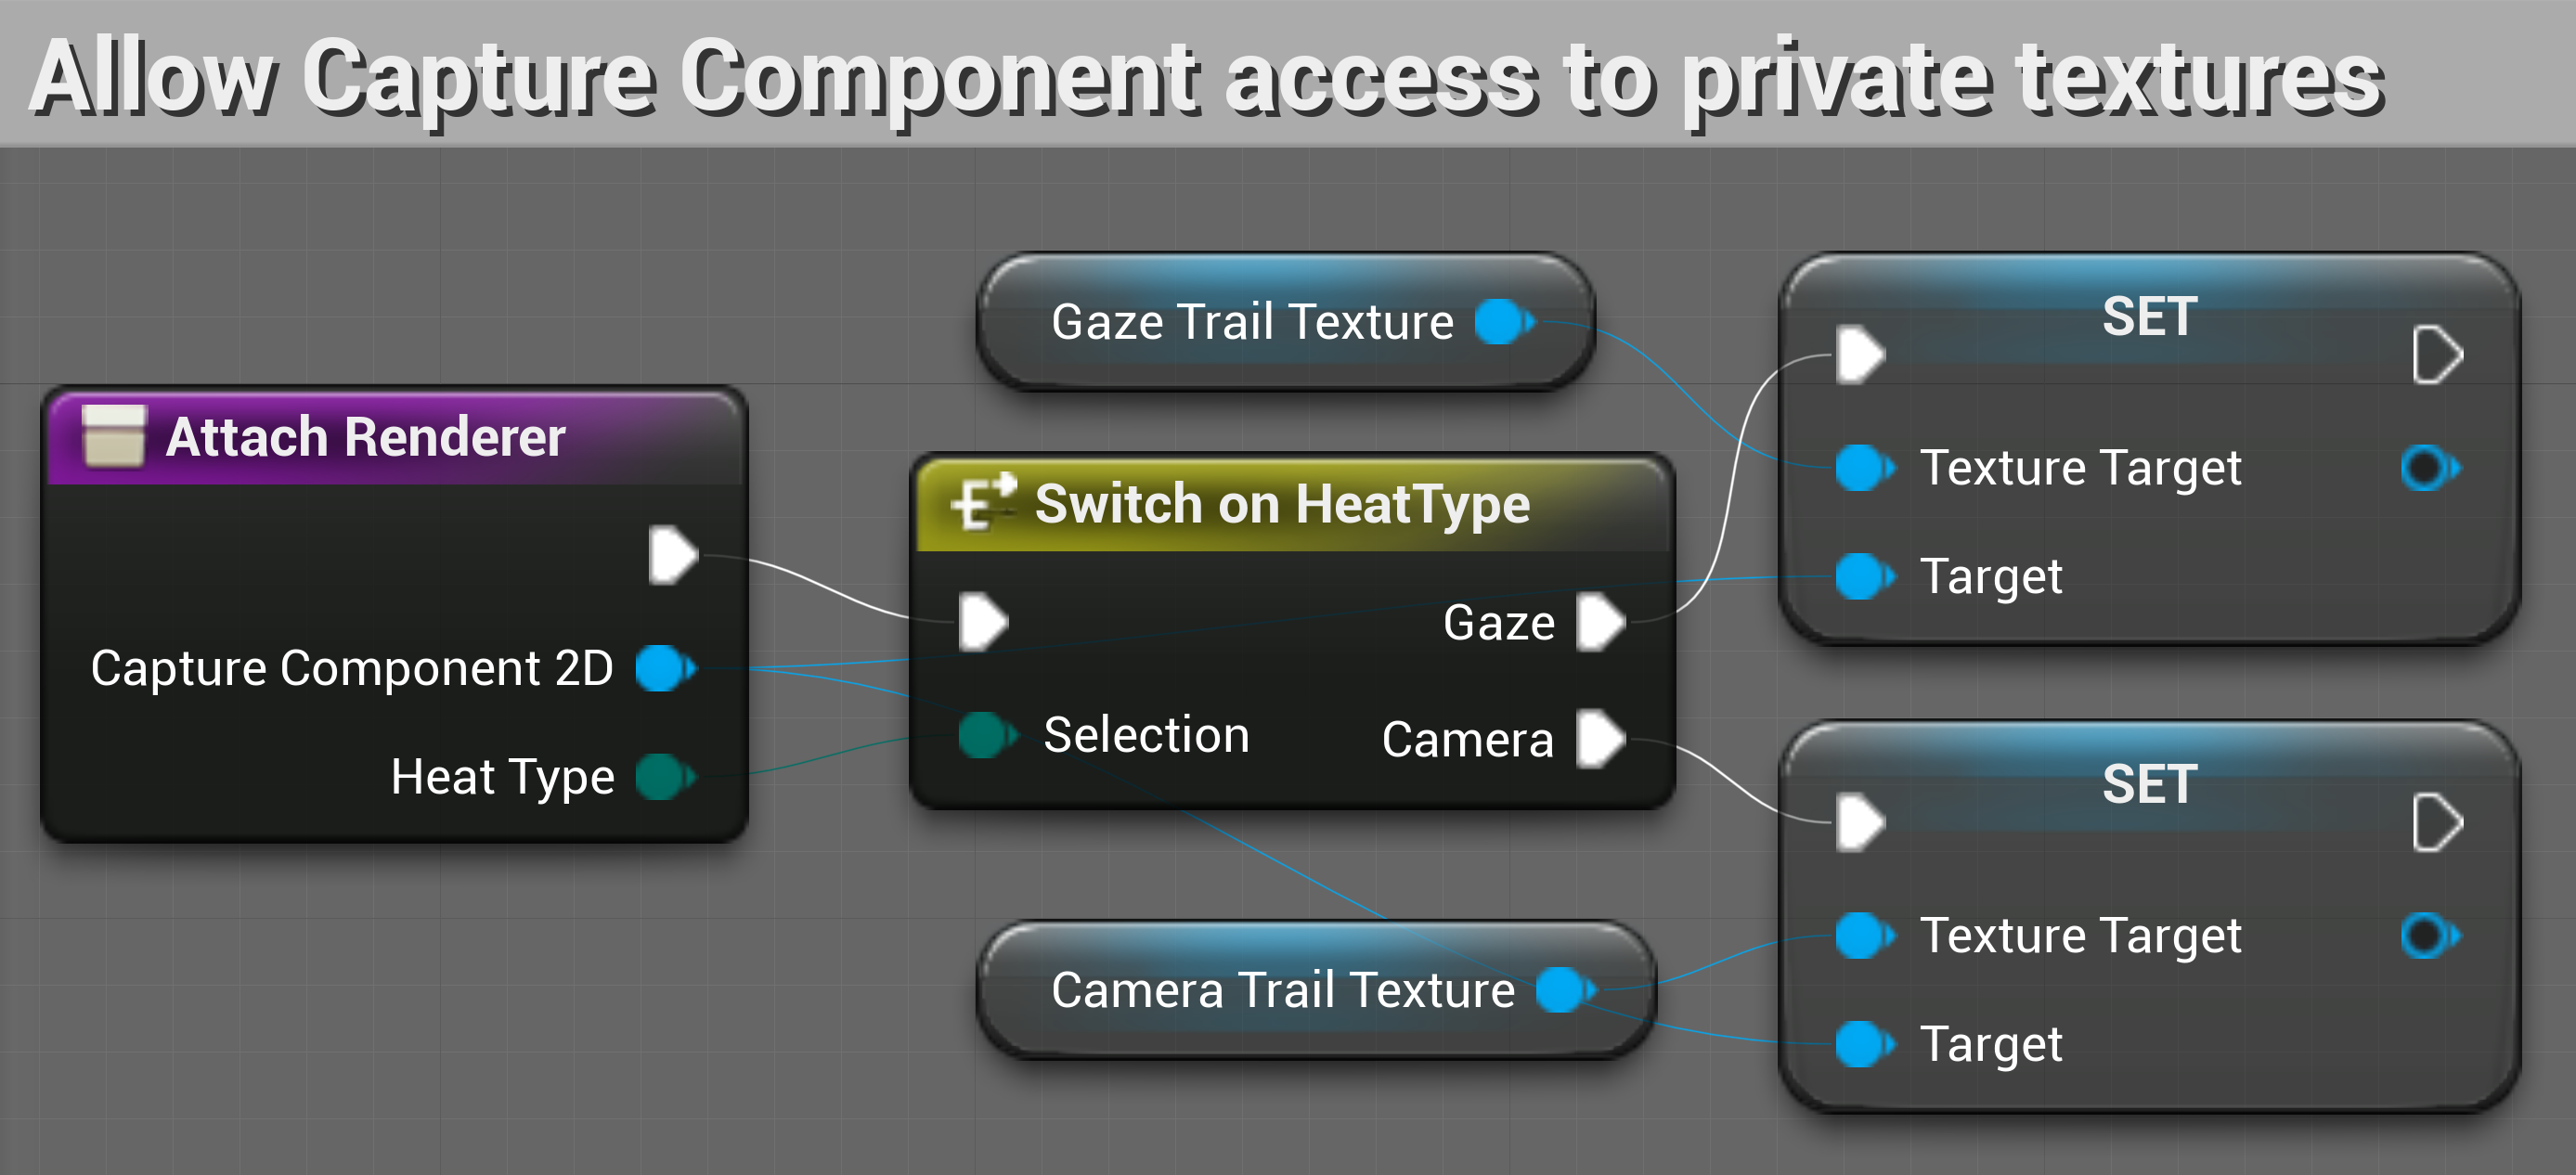
\includegraphics[width=0.6\textwidth]{img/attach-renderer.png}
    \caption{AttachRenderer function in EyeTrackedStaticMeshComponent.}
    \label{fig:attach-renderer}
\end{figure}

\begin{figure}[!ht]
    \centering
    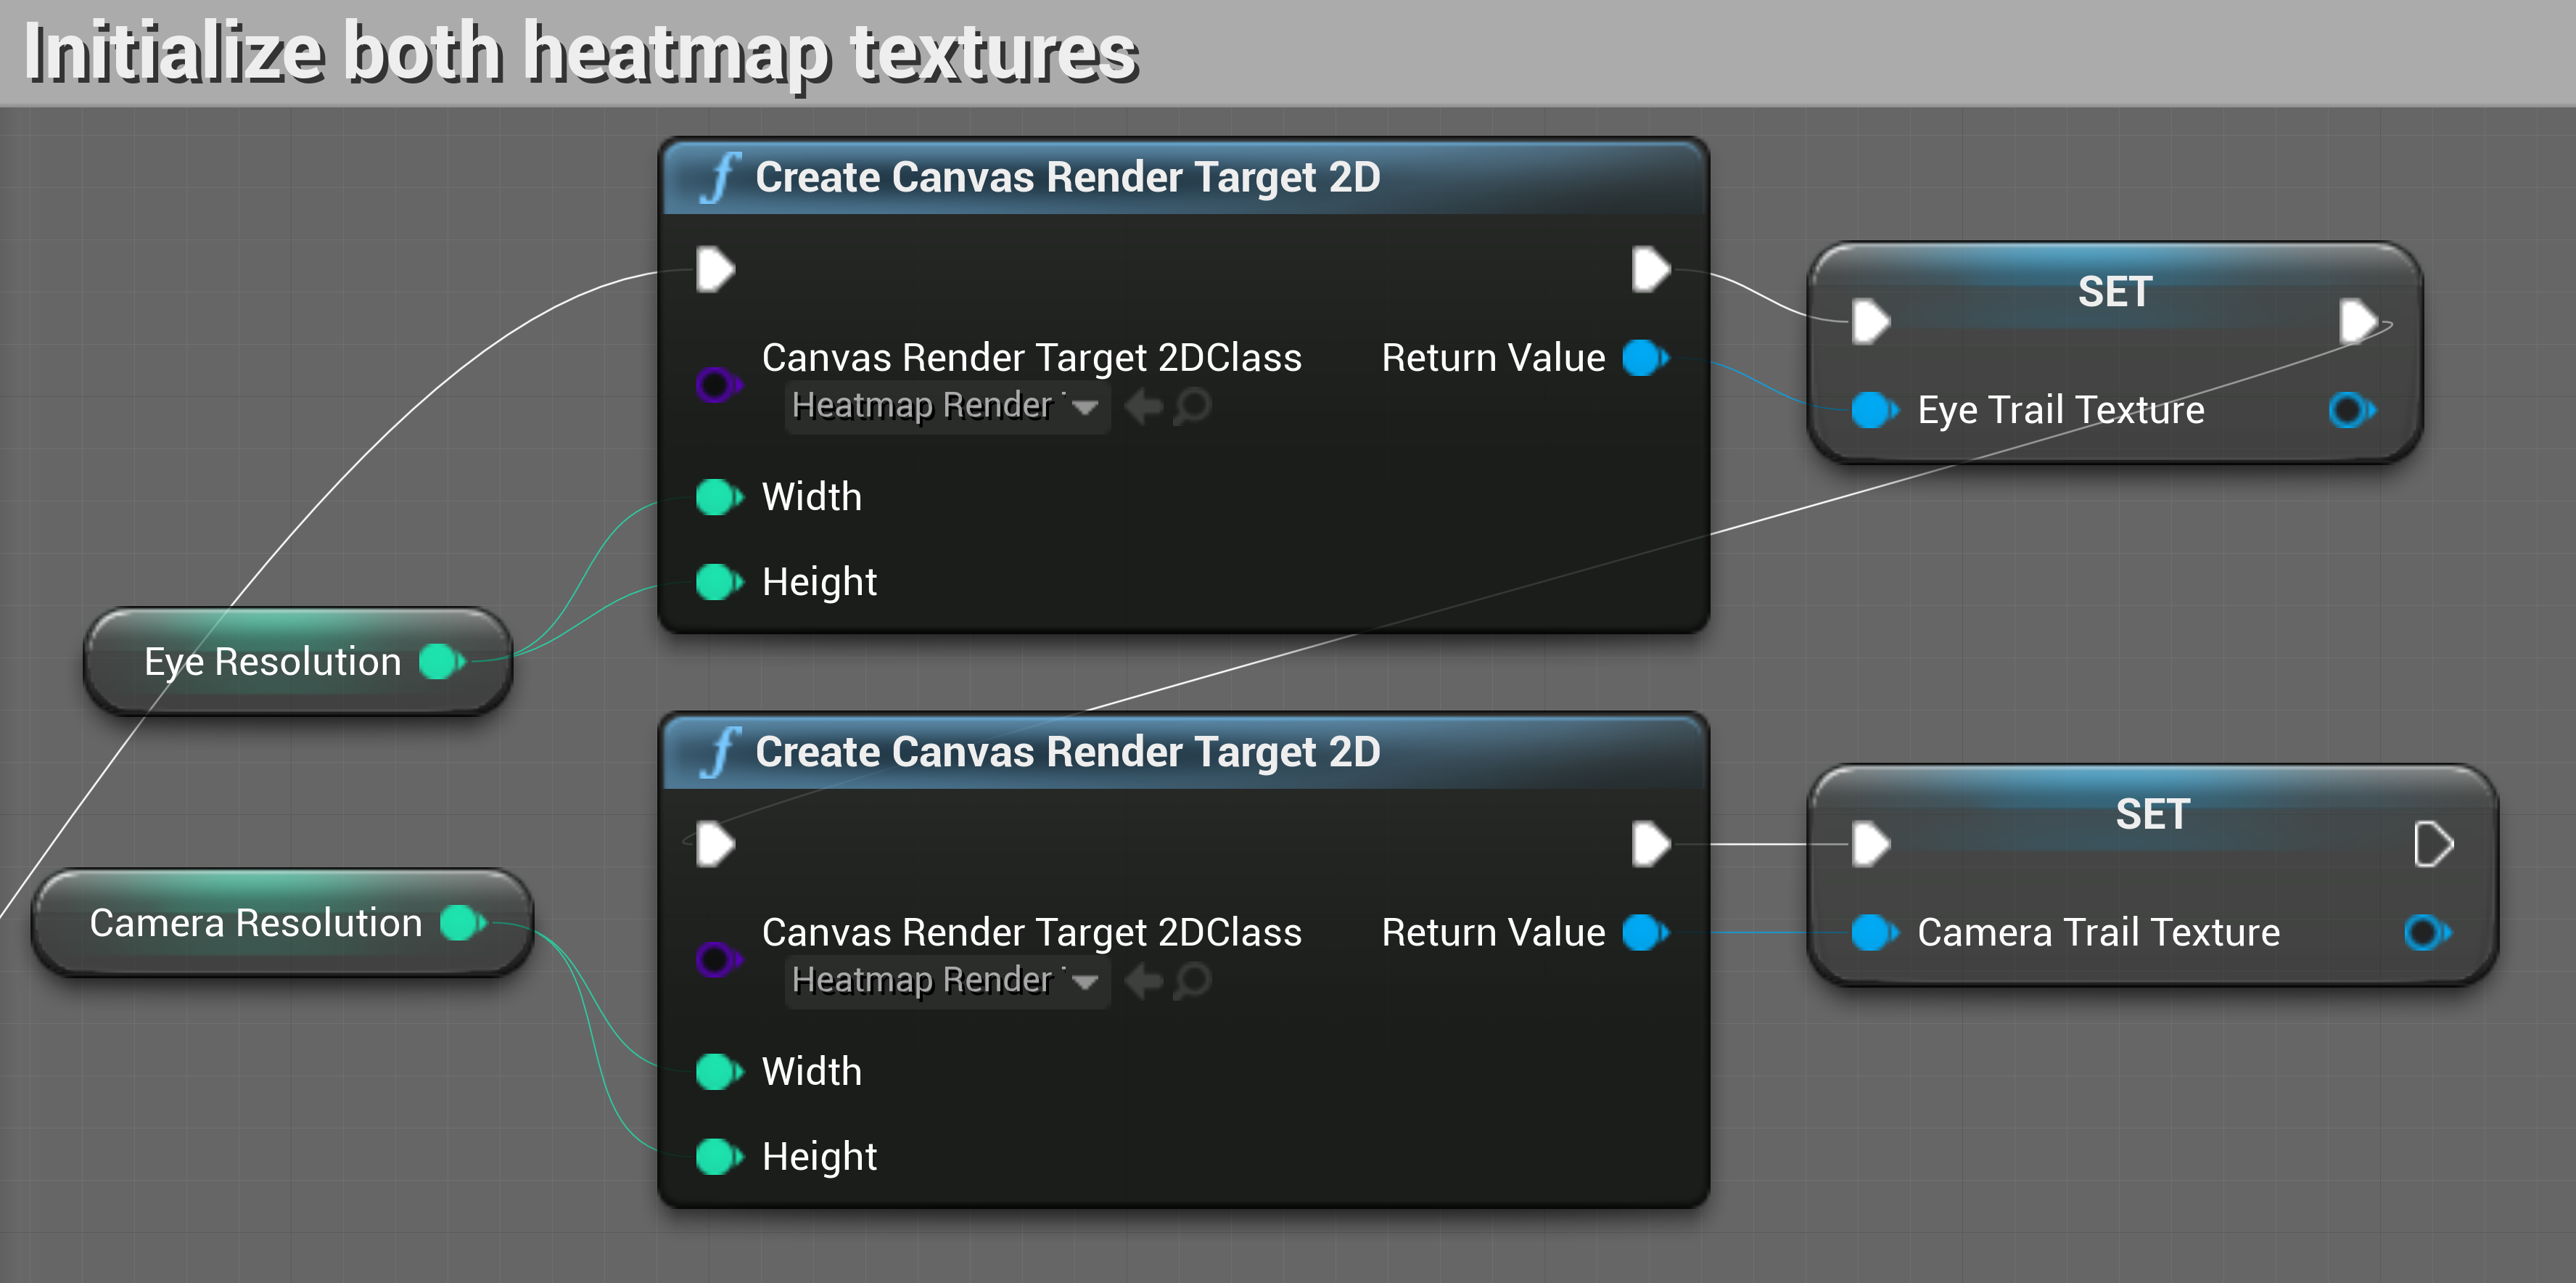
\includegraphics[width=\textwidth]{img/ETcomponent-init.png}
    \caption{EyeTrackedStaticMeshComponent render target initialisation.}
    \label{fig:RT-init}
\end{figure}

\pagebreak{}

\subsubsection*{Texture file operations}
Another key function of this component is the~export and import of heatmap textures. The~format is RGBA with 16-bit colour depth for higher accuracy of the~measured heatmaps. For this type of texture, the~EXR format was chosen. Unreal Engine offers disk input and output operations in this format. The~reason for choosing it was that EXR-format images can be exported and imported using the~OpenEXR library for Python~\cite{openexr}, which will be useful for later image processing.

The~whole export depends only on creating a~file path and calling the~\emph{ExportToDisk} Blueprint function, which takes the~export options as a~pin. There, it is possible to choose the~texture export format and the~compression rate; Figure~\ref{fig:export-heatmaps-exr}. The~path to the~file is created by simple string operations shown in Figure~\ref{fig:make-filepath}. The~comment of these nodes also contains the~format of the~path that the~operations create. In total, two paths are created. One for the~gaze heatmap and one for the~camera heatmap.

The~loading depends first on loading the~image file itself by calling the~\emph{Import File as Texture2D} function and passing the~filename parameter. 
The~procedure for passing this texture object to an~editable render target can be seen in Figure~\ref{fig:load-heatmap-textures}. A~new dynamic material instance of LoadMaterial is created. This material is given a~texture parameter with the~value of the~loaded texture object to be rendered by the~\emph{Draw Material To Render Target} function.

\subsubsection*{EyeTrackingHelperLibrary}

This is a~static library with Load, Export, and Toggle functions that take care of iterating through all EyeTrackedStaticMeshComponents in the~scene and then calling their respective functions individually.

\begin{figure}[!ht]
    \centering
    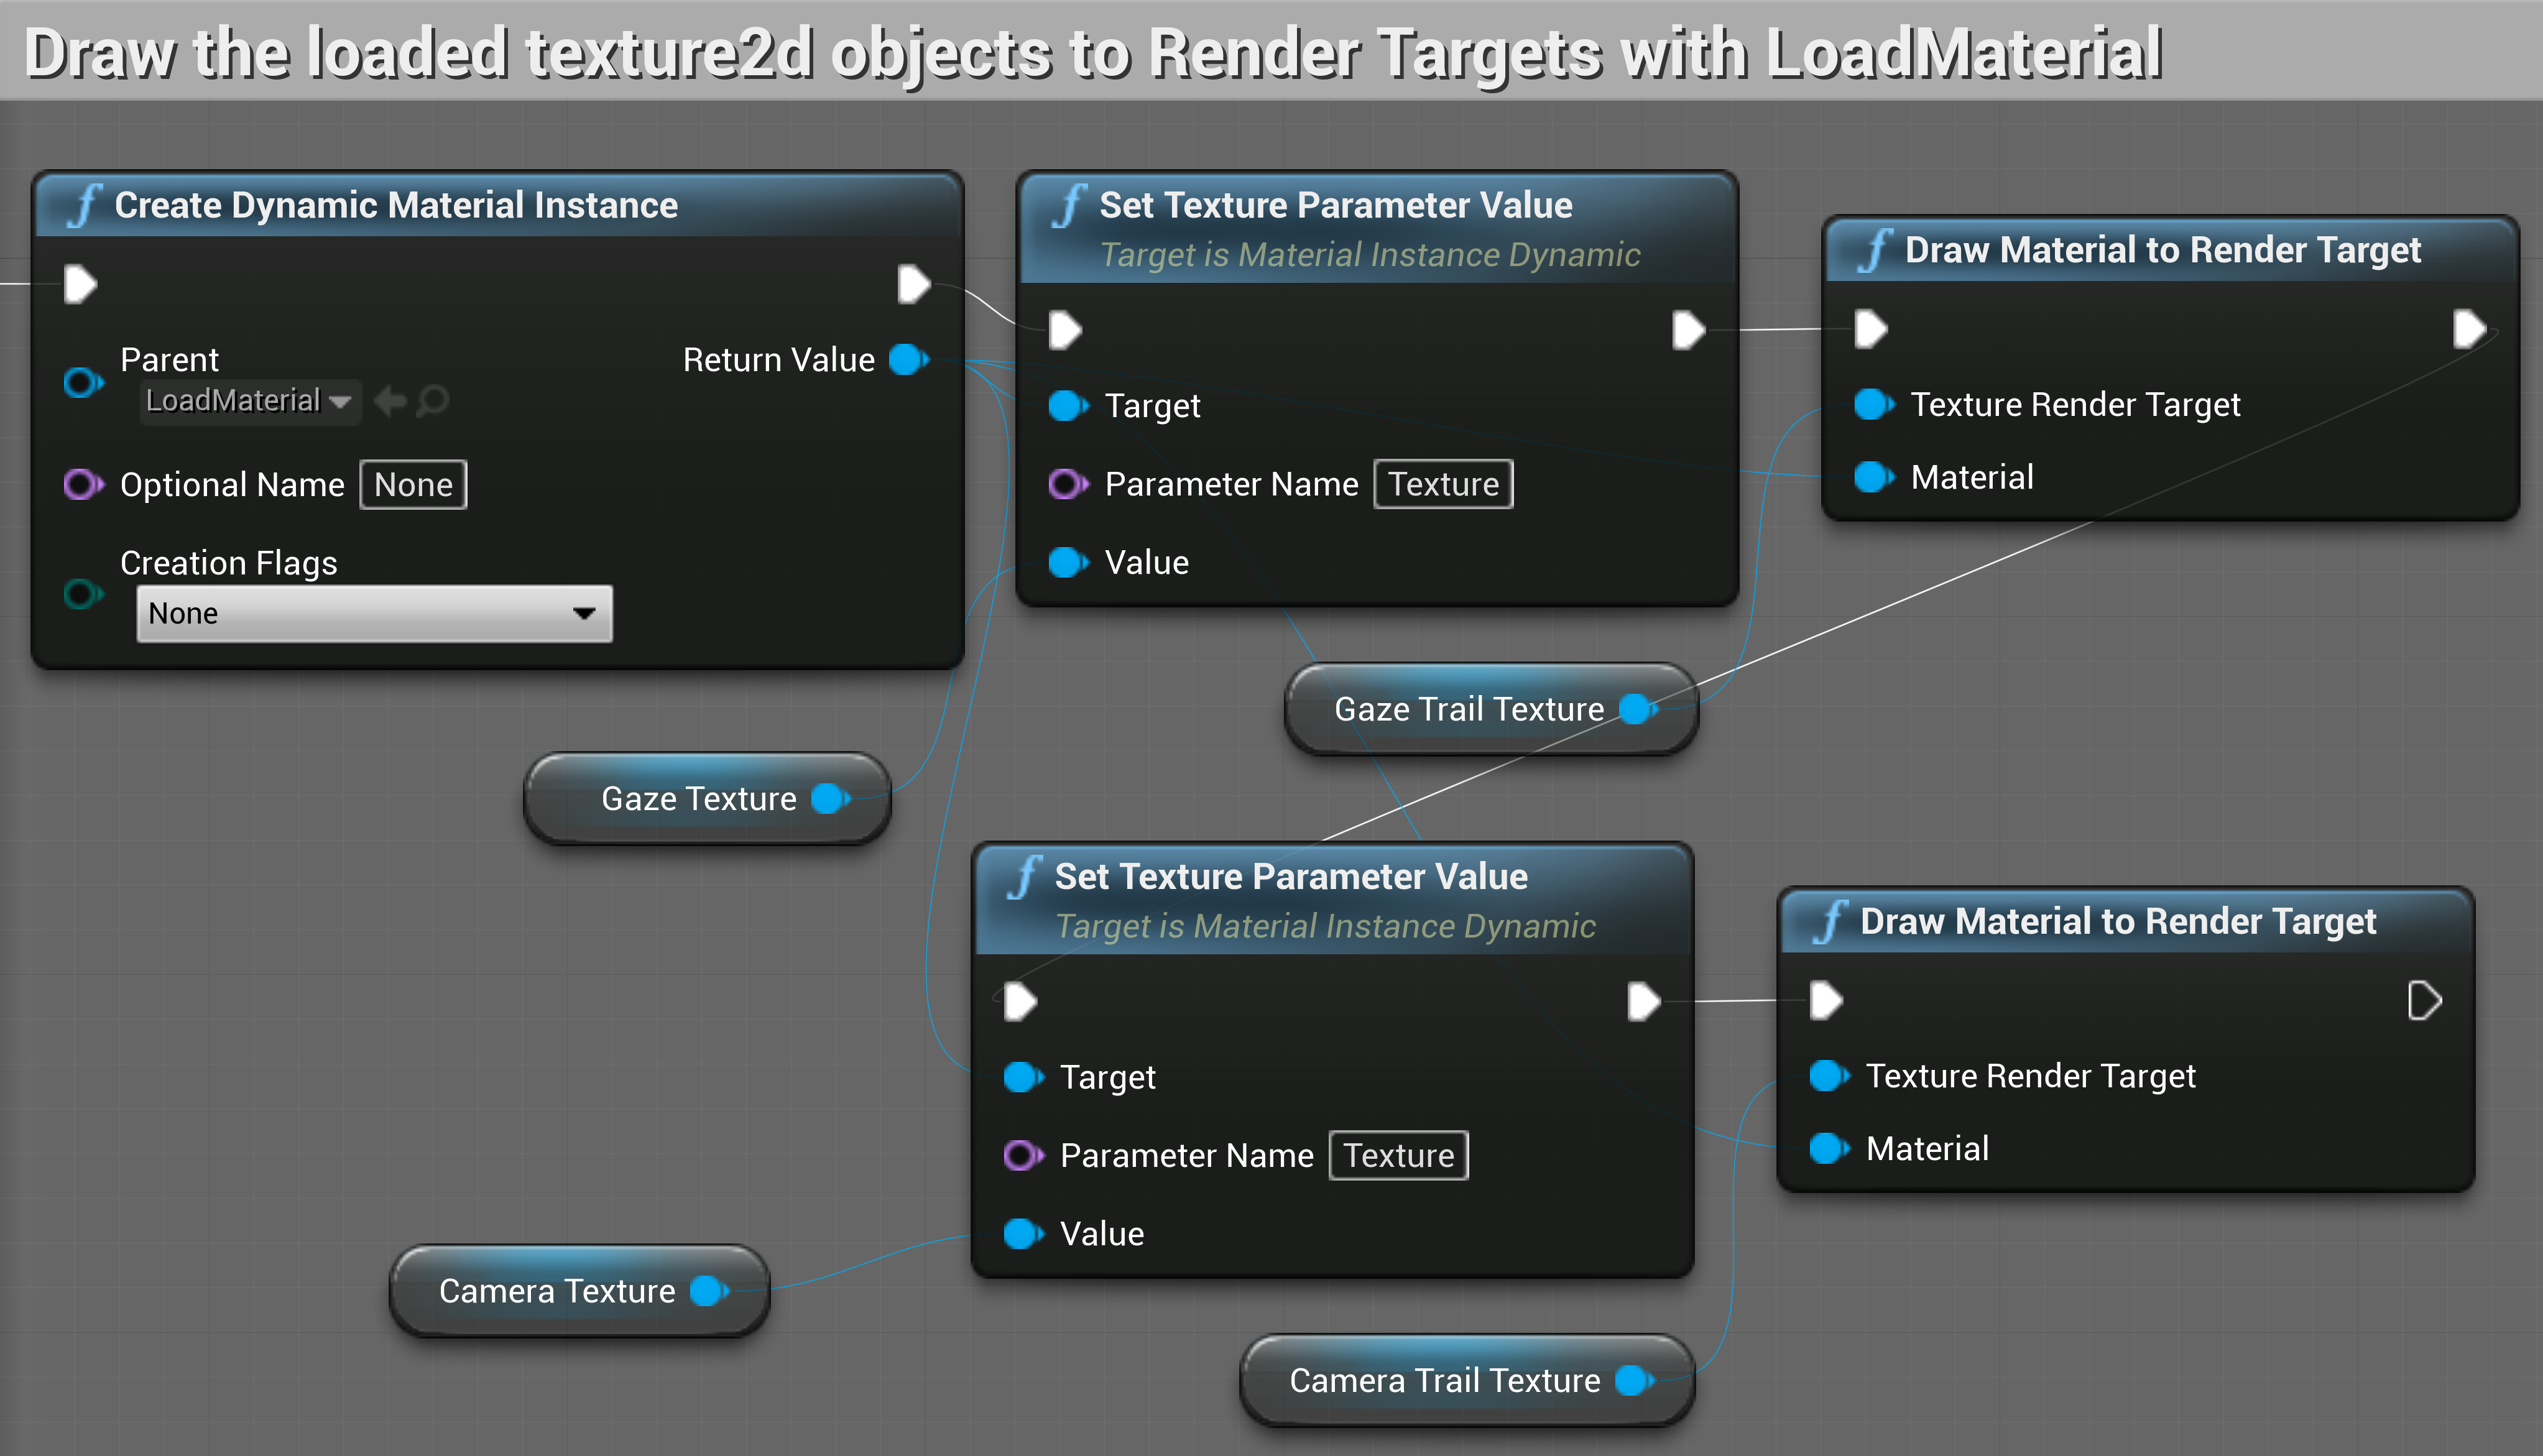
\includegraphics[width=\textwidth]{img/load-heatmap-textures.png}
    \caption{Loading heatmap textures to render targets.}
    \label{fig:load-heatmap-textures}
\end{figure}

\pagebreak{}

\begin{figure}[!ht]
    \centering
    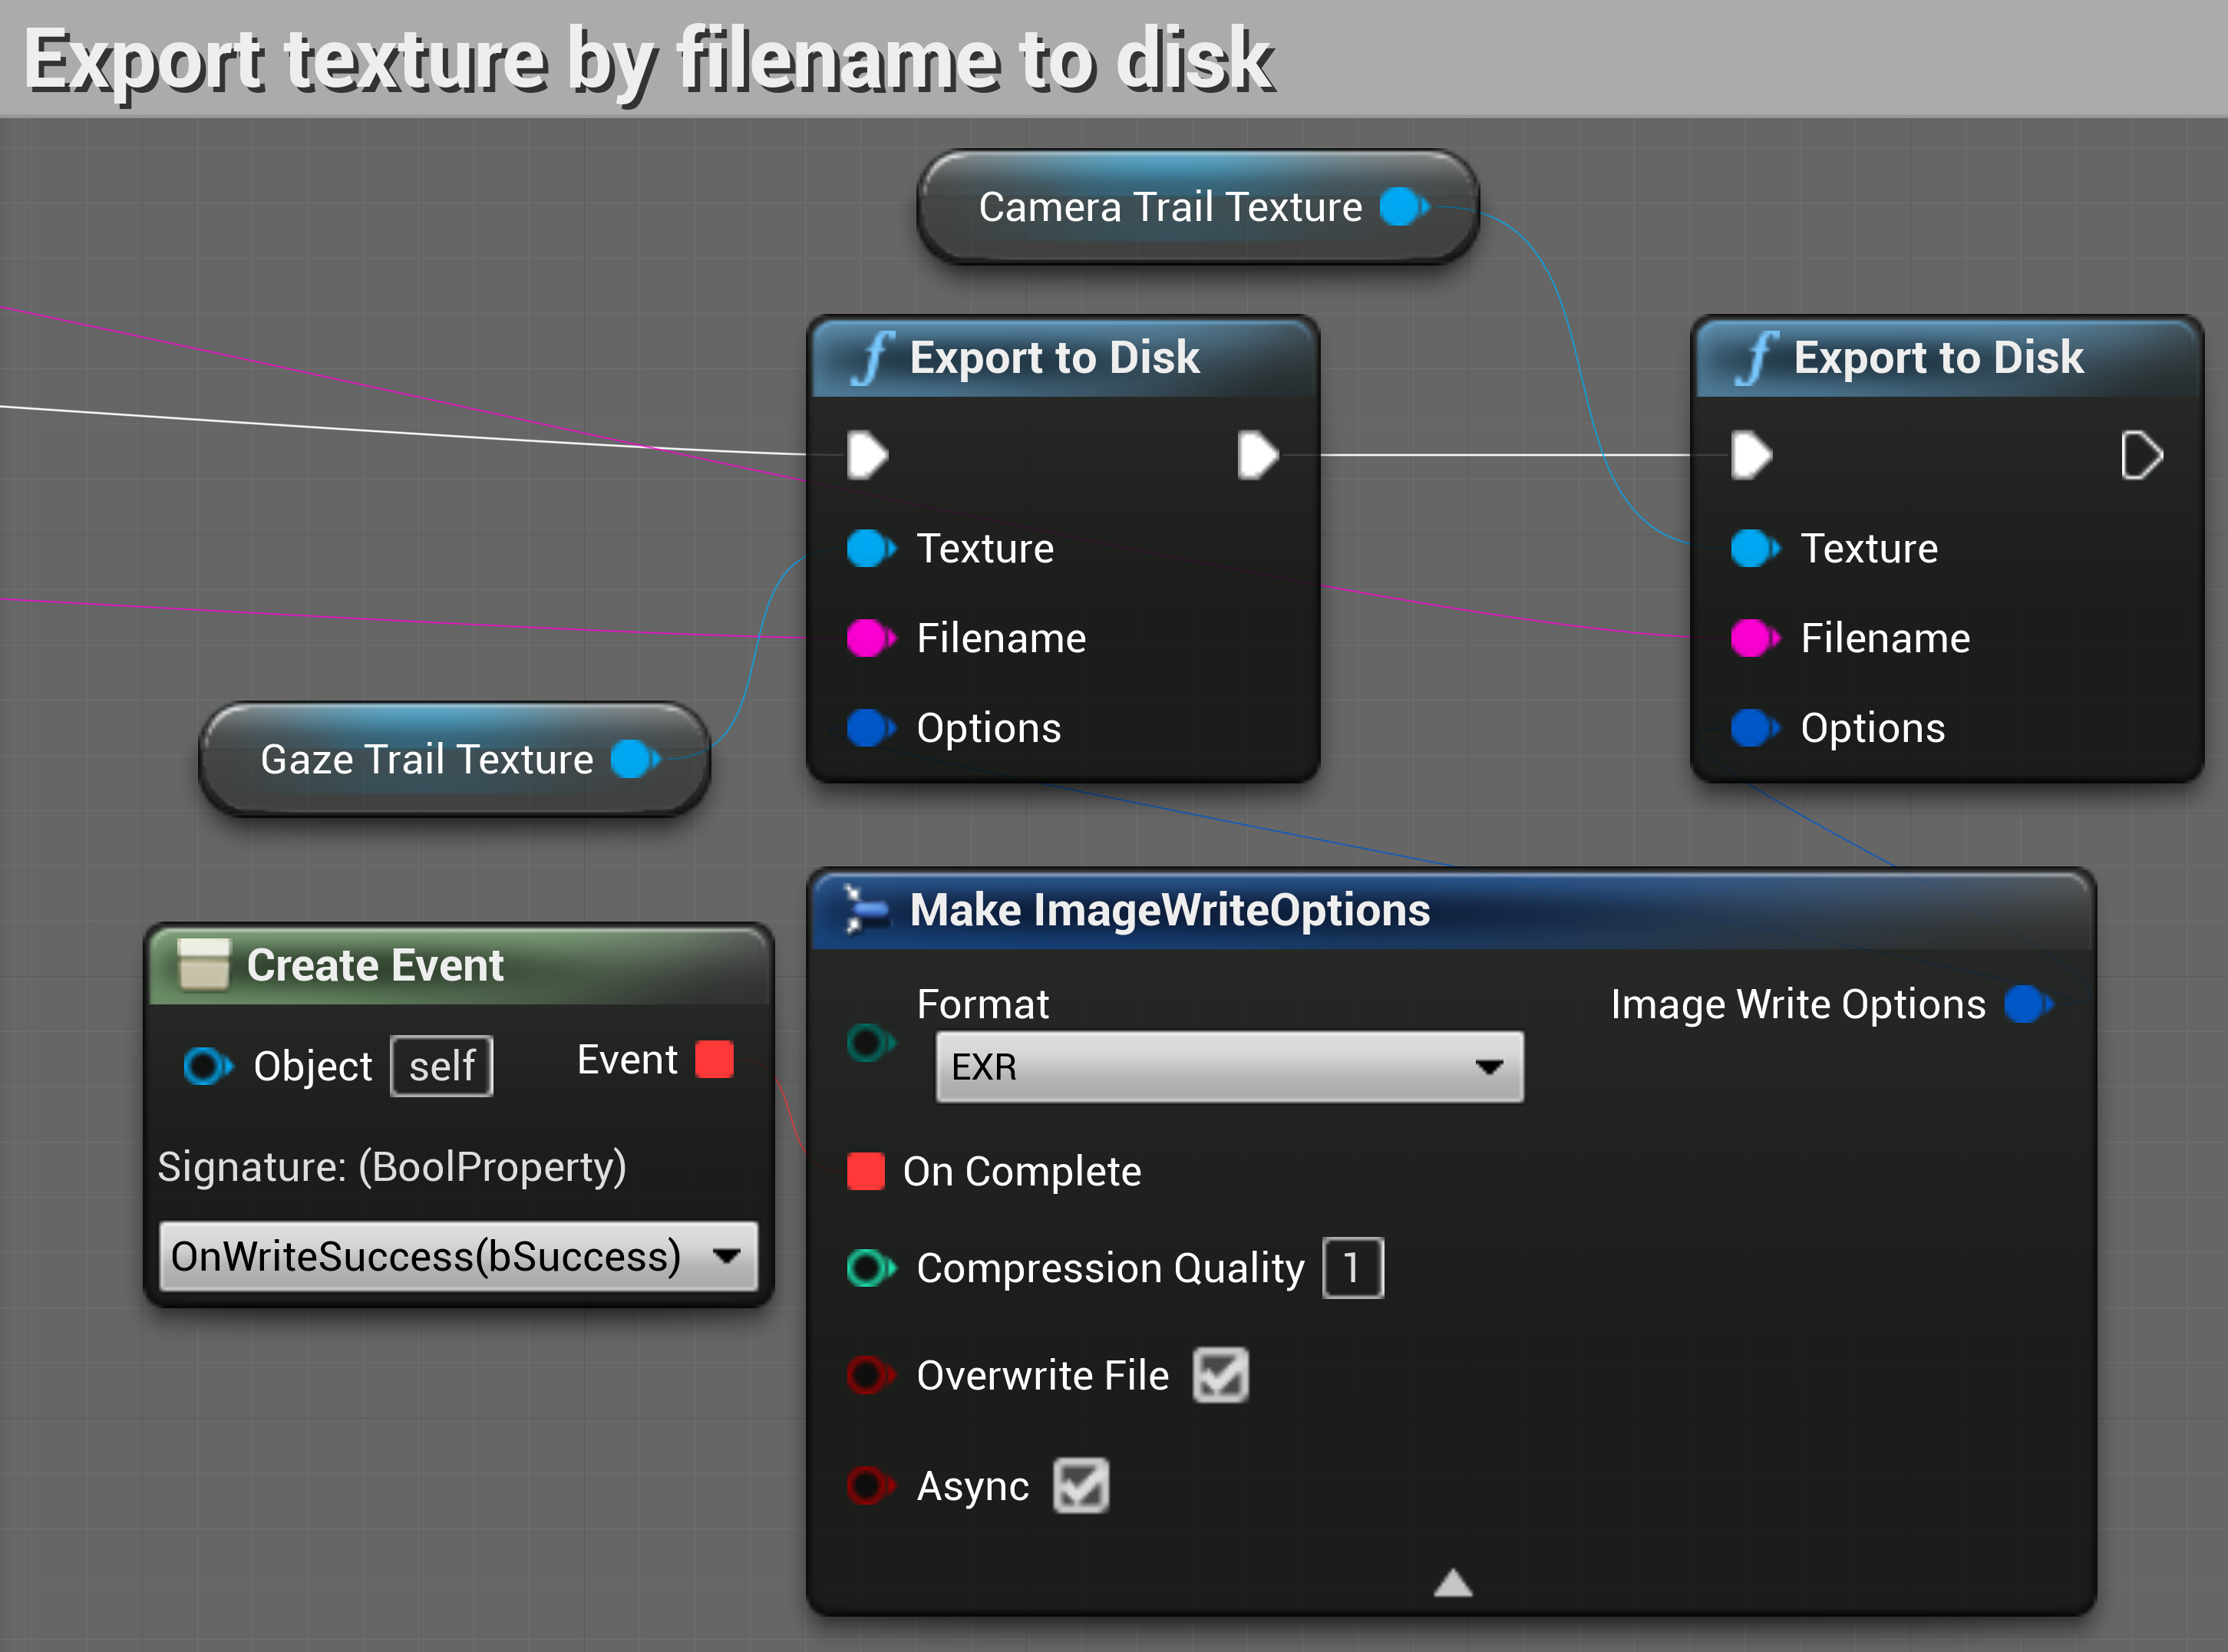
\includegraphics[width=\textwidth]{img/export-both-heatmap-textures.png}
    \caption{Export gaze and camera heatmap textures as EXR image format.}
    \label{fig:export-heatmaps-exr}
\end{figure}

\begin{figure}[!ht]
    \centering
    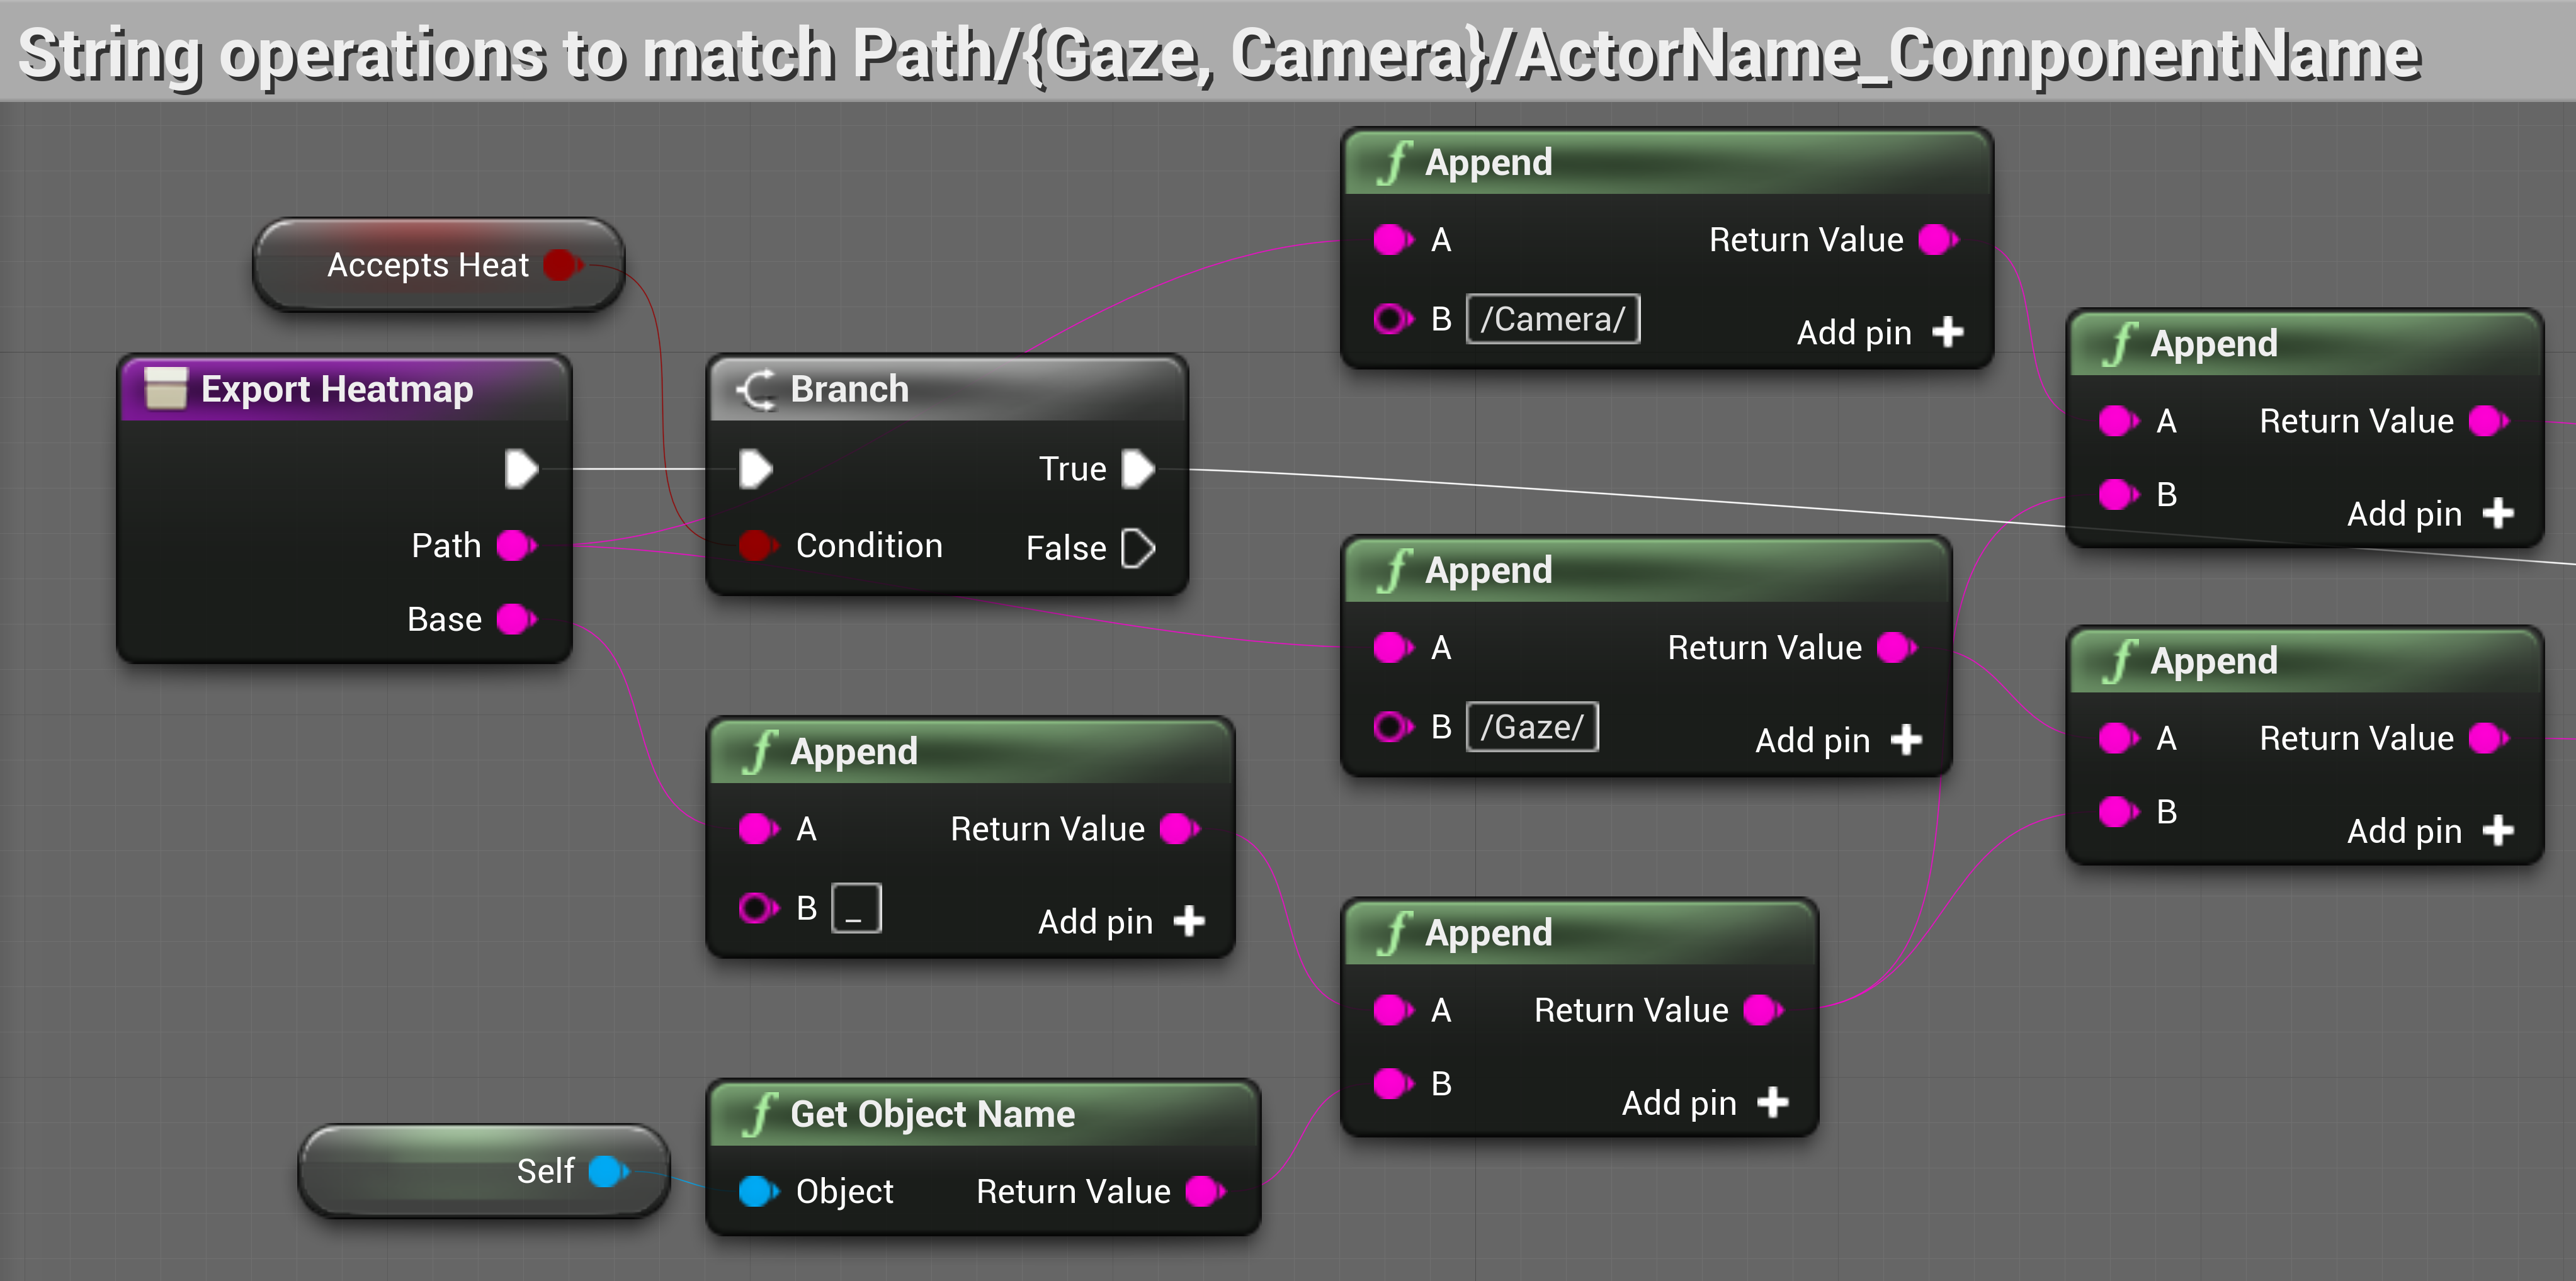
\includegraphics[width=\textwidth]{img/make-texture-filepath.png}
    \caption{Make filepath for the~exported gaze and camera heatmap textures.}
    \label{fig:make-filepath}
\end{figure}

\pagebreak{}

\subsection{HeatmapProducer}
\label{sec:uv-unwrap-implementation}
This class is used to produce heatmaps. Its design is based on the~analysis in Section~\ref{sec:uv-unwrap-method}. The~blueprint for recording unwrapped meshes is inspired by Tran's tutorial~\cite{tran2018wenderlich}. In order to function, it is absolutely necessary to insert this Actor into the~scene.

\begin{figure}[!ht]
    \centering
    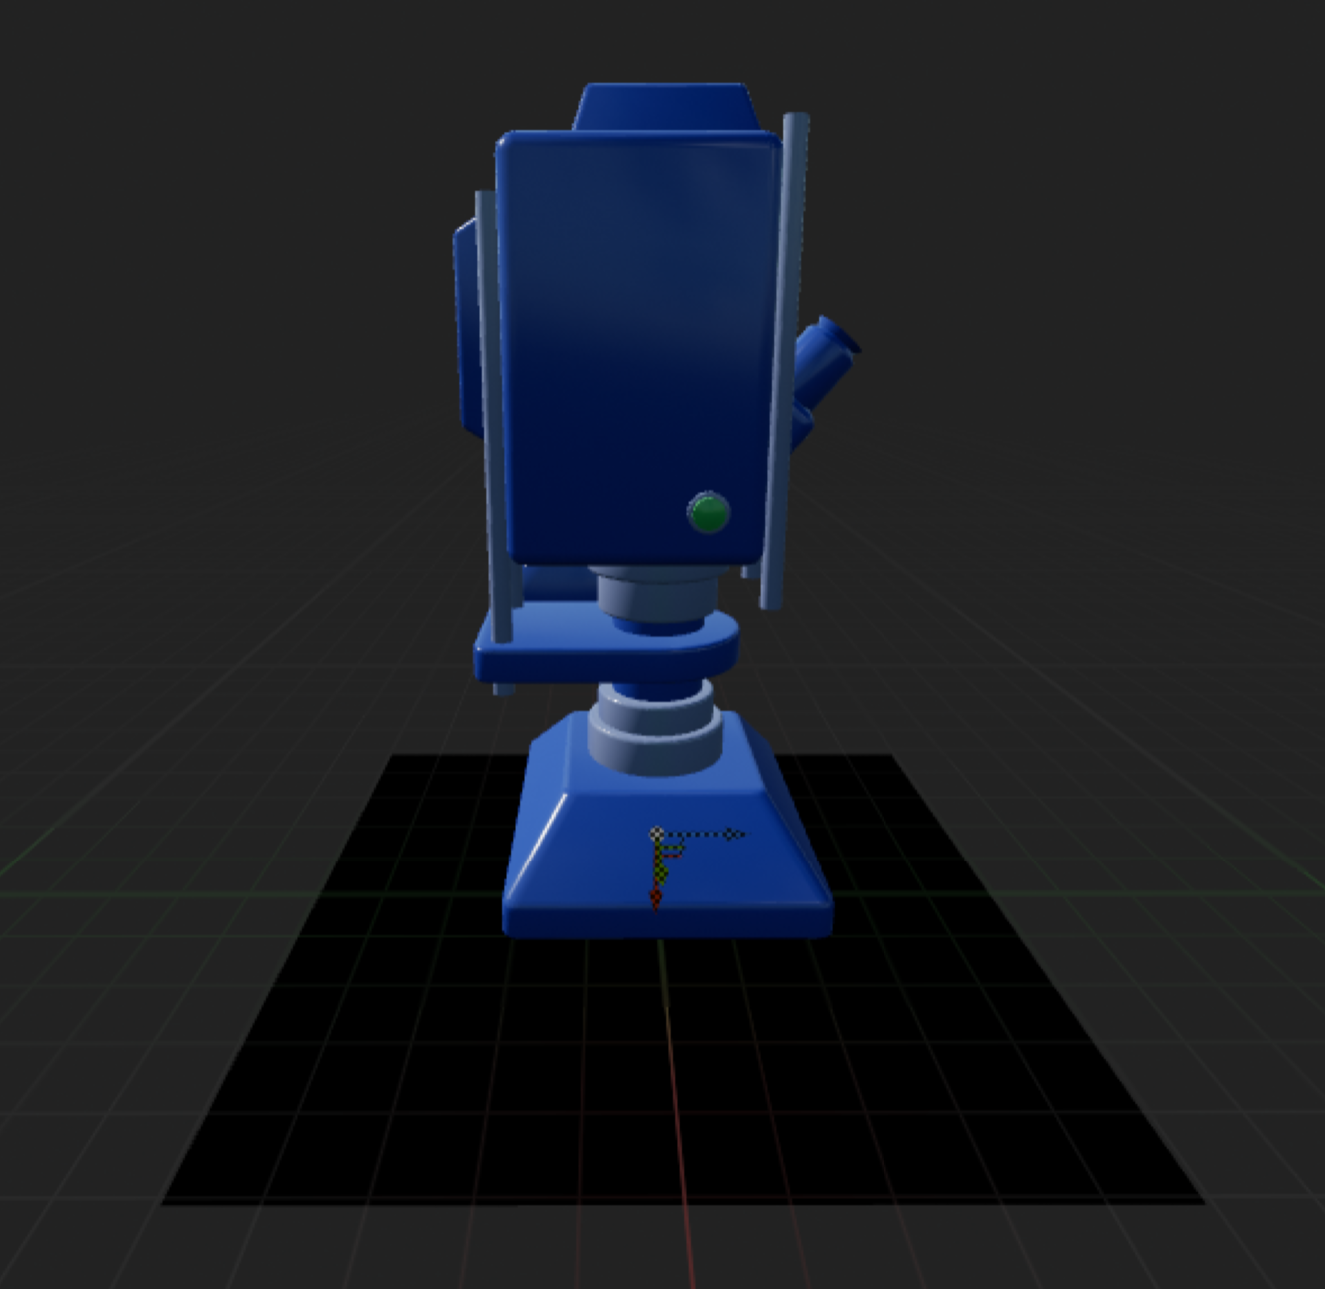
\includegraphics[width=0.4\textwidth]{img/heatmap-producer-viewport.png}
    \caption{HeatmapProducer capture component with background plane in viewport.}
    \label{fig:heatmap-producer-viewport}
\end{figure}

First, it is important to describe what the~Actor consists of. To record a~static mesh that unwraps itself into the~world according to its UV map, it is necessary to record the~state of this model with some kind of camera. This is what the~Scene Capture Component, with the~name of \emph{UnwrapUVCapture}, is for. To avoid recording unwanted effects from ambient lights and occlusion, the~camera is paired with a~simple plane to which a~UVRenderBackground material is added, which creates a~black background for the~mesh, as shown in Figure~\ref{fig:heatmap-producer-viewport}. The~camera is rotated $270{^\circ}$ on the~$z$ and $y$ axes to point directly at the~background. It is positioned higher than the~background, which is shifted to negative values of the~$z$-axis to avoid z-fighting with an~unwrapped mesh.  

The~capture component settings can be seen in Figure~\ref{fig:capture-component-settings}. The~camera must be of orthographic type and its width must correspond exactly to the~size of the~background plane. It is also critical to set the~Composite Mode to Additive, to ensure that capturing the~scene does not overwrite previous values but adds them to a~texture. The~background is a~square with a~100 cm long edge.

\begin{figure}[!ht]\centering
    \begin{subfigure}[b]{0.495\textwidth}
        \centering
        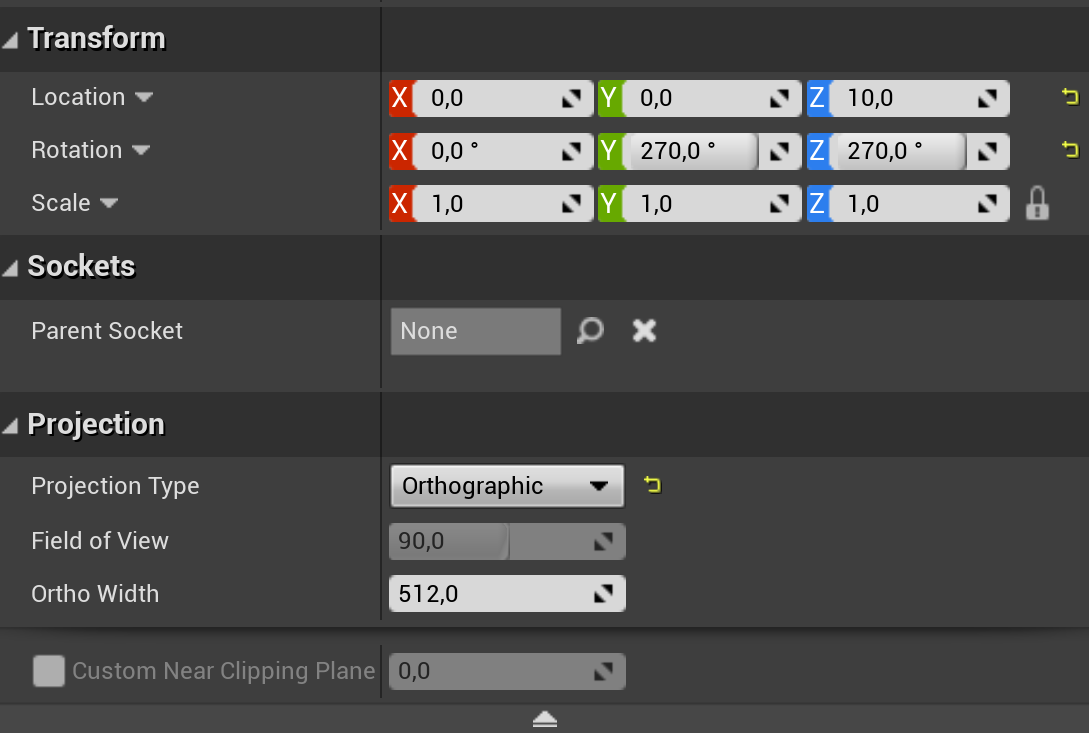
\includegraphics[width=\textwidth]{img/capture-component-settings.png}
    \end{subfigure}
    \hfill
    \begin{subfigure}[b]{0.495\textwidth}
        \centering
        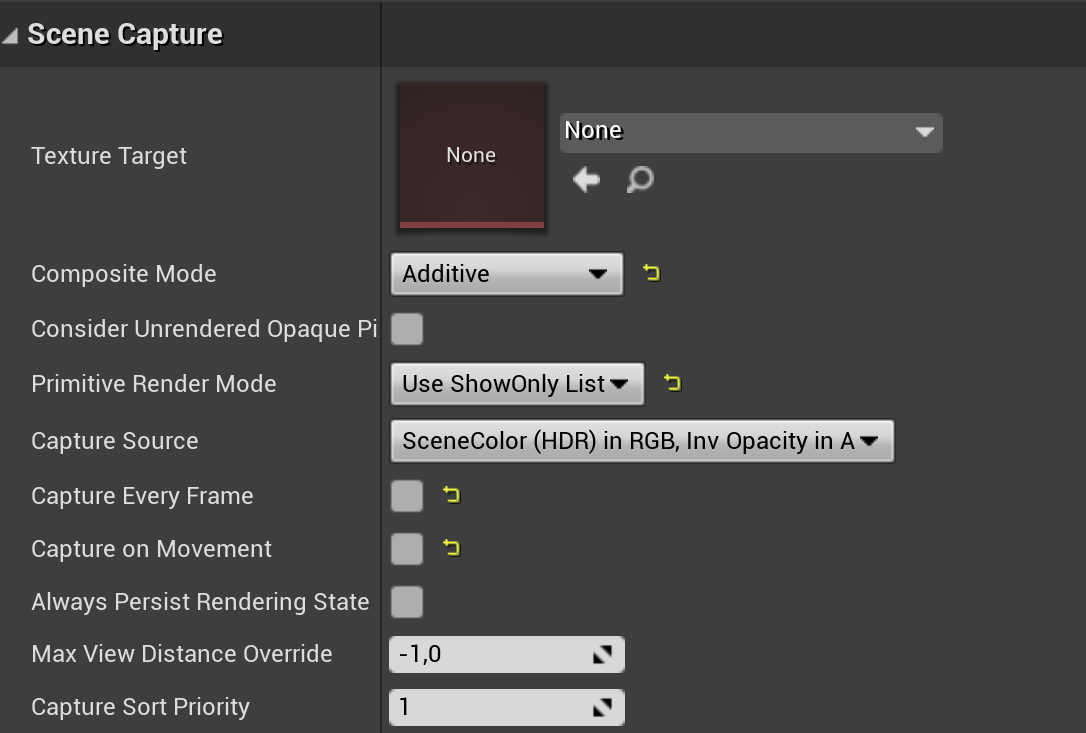
\includegraphics[width=\textwidth]{img/scene-capture-settings.png}
    \end{subfigure}
    \caption{UnwrapUVCapture Component settings.}
    \label{fig:capture-component-settings}
\end{figure}

\pagebreak{}

The~HeatProducer Actor contains a~private variable of the~dynamic material instance of UnwrapBrush material that is initialised in the~construction script of this Actor. Its parameters are described in Sections~\ref{sec:uv-unwrap-method} and \ref{sec:unwrap-brush-implementation}.

\subsubsection*{AlignRenderer function}

This function takes as input the~texture resolution and the~world position of an~unwrapped mesh. It is used to align the~two components of the~Actor and UnwrapBrush dynamic material instance parameters based on texture size and world position; that is, to avoid object culling, Section~\ref{sec:uv-unwrap-method}. To capture a~mesh into a~texture correctly, the~ortho width of the~capture component must first be set to the~exact resolution of the~texture. The~background must have its scale values on the~$x$ and $y$ axes adjusted to $t/100$, where $t$ is the~texture resolution in pixels, to be exactly the~same size as the~ortho width.

The~texture resolution is uploaded to the~dynamic material via the
\emph{CaptureSize} parameter and the~3D location of the~unwrapped object via the~\emph{UnwrapLocation} parameter.

\subsubsection*{PrepareScene}
The~PrepareScene function just takes an~EyeTrackedStaticMeshComponent and includes it along with the~black background in the~empty show-only list of the~capture component. 

\subsubsection*{ApplyHeatToComponent}

This function takes care of preparing the~HeatProducer Actor and the~component for rendering. As Figure~\ref{fig:apply-heat-function} shows, the~black background is first made visible, since it is normally not, then AlignRenderer is called according to the~resolution, the~PrepareScene function immediately after, and finally the~RenderSplatOntoComponent is called to render the~heatmap. It finishes by making the~background invisible again. 

\begin{figure}[!ht]
    \centering
    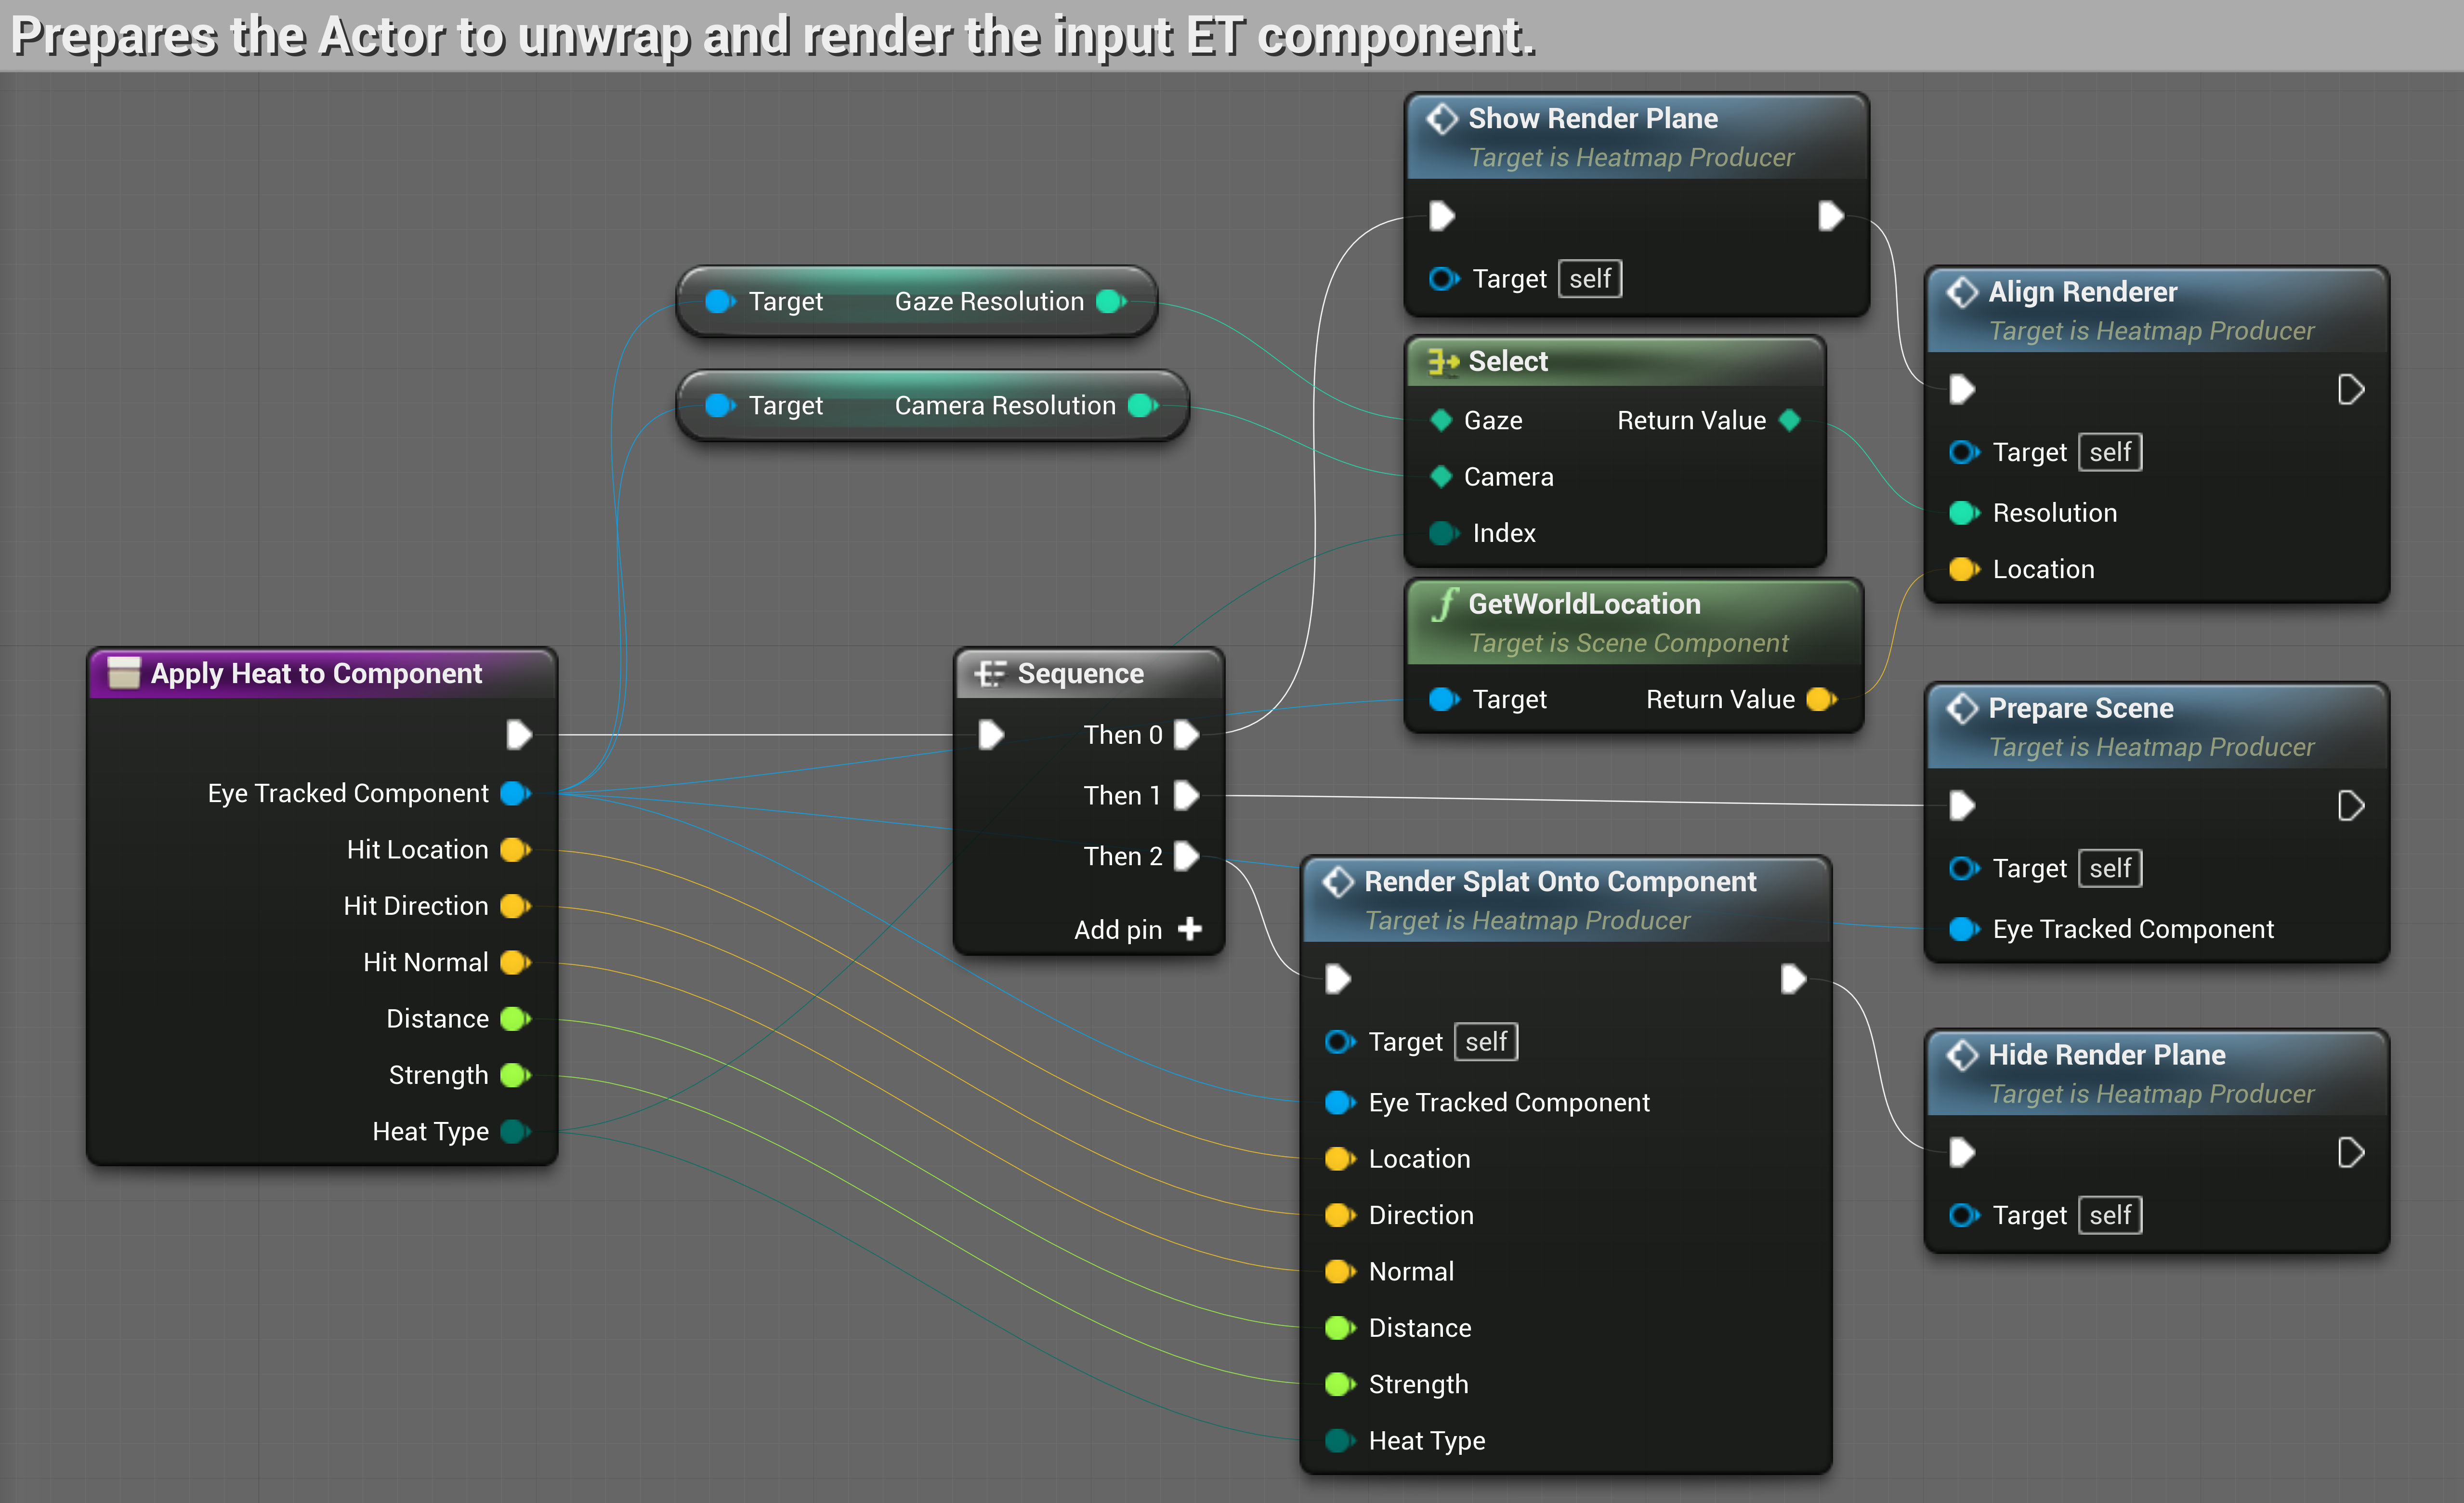
\includegraphics[width=\textwidth]{img/apply-heat-to-component.png}
    \caption{HeatmapProducer ApplyHeatToComponent function.}
    \label{fig:apply-heat-function}
\end{figure}

\subsubsection*{RenderSplatOntoComponent}

This is a~function of many inputs. Namely, Location, Direction (from camera), Normal, Distance, and Strength. All of them correspond to all the~remaining parameters of the~UnwrapBrush material, which are set exactly as the~previous cases of dynamic material parameters, for example, Figure~\ref{fig:load-heatmap-textures}. These are HitLocation, DirectionToCamera, HitNormal, BrushRadius, and Strength.

Next, the~original material of the~component is stored in a~local variable, because its material is immediately replaced by the~UnwrapBrush instance. This can be seen in Figure~\ref{fig:render-splat-function}. Thus, it is immediately rendered, after a~render target has been assigned to it, using the~Capture Scene function. At this point, a~new value is added to the~render target according to UnwrapBrush. The~function ends by returning the~component its original material. 

\begin{figure}[!ht]\centering
    \begin{subfigure}[b]{\textwidth}
        \centering
        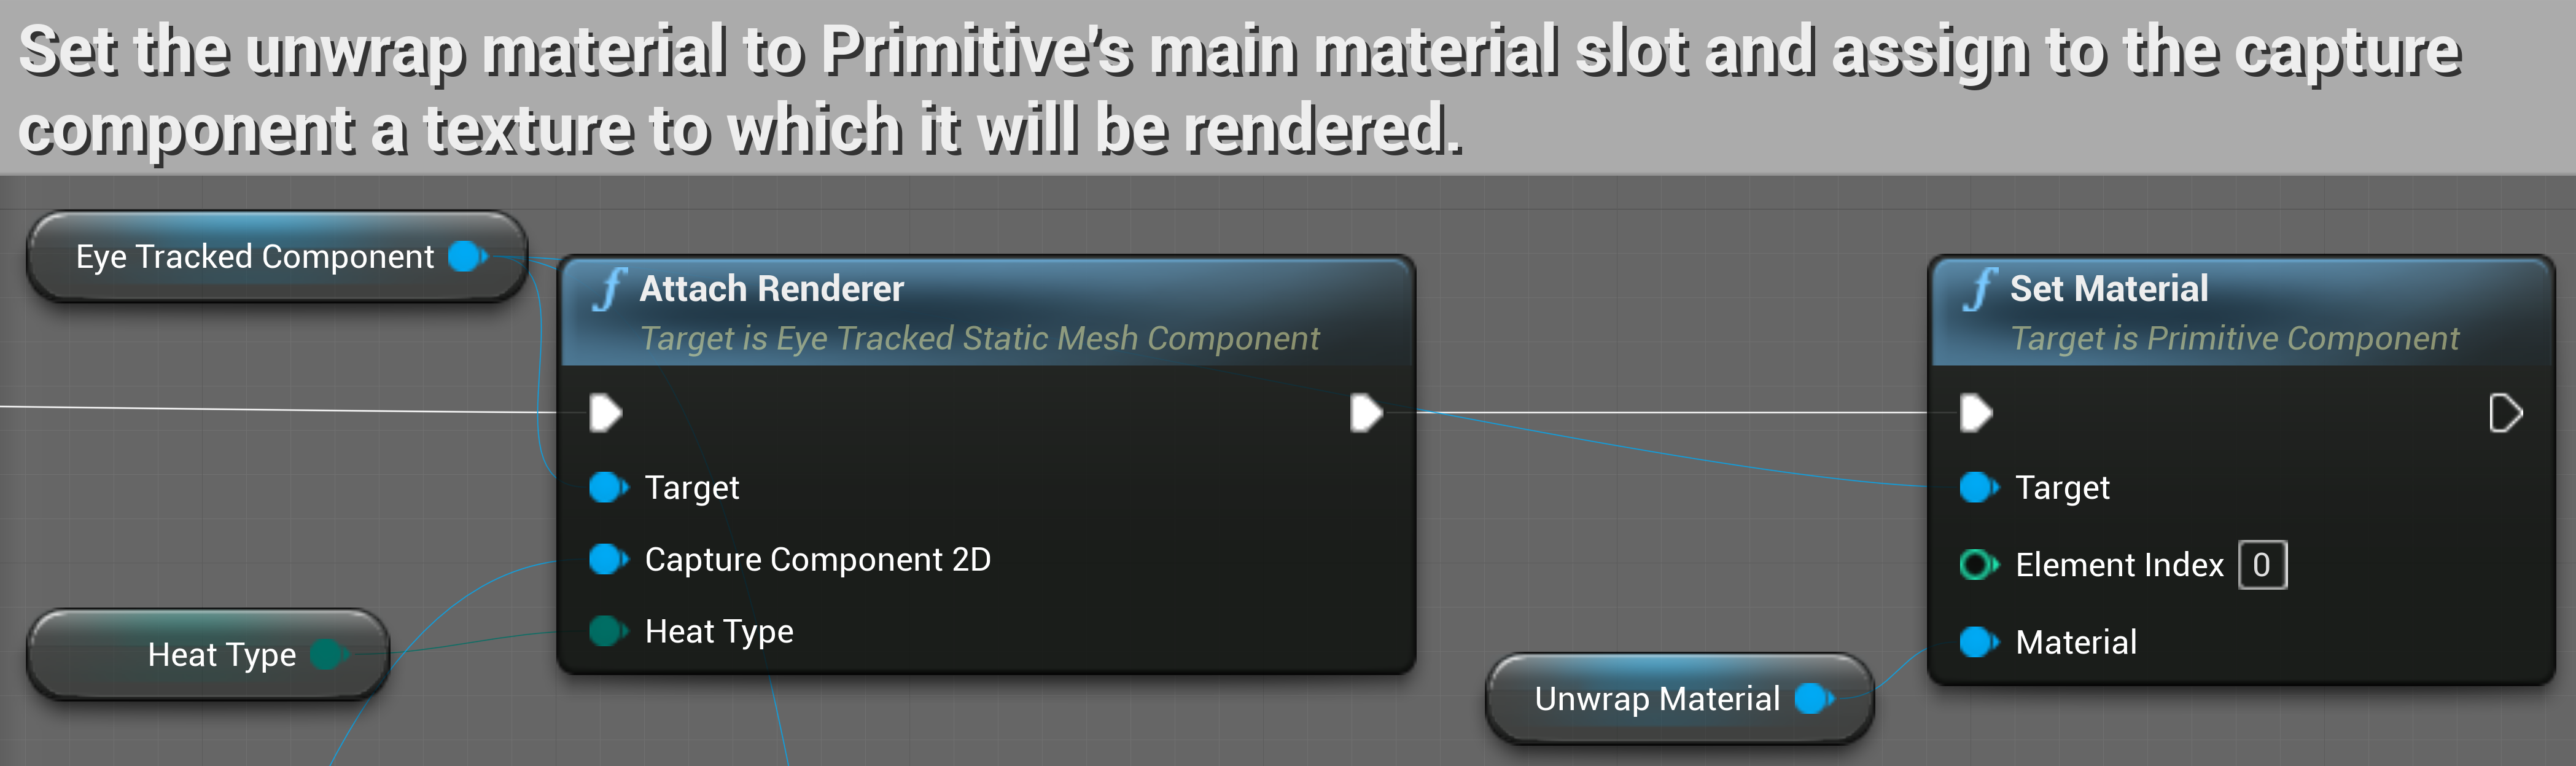
\includegraphics[width=\textwidth]{img/render-splat-1.png}
    \end{subfigure}
    \hfill
    \begin{subfigure}[b]{\textwidth}
        \centering
        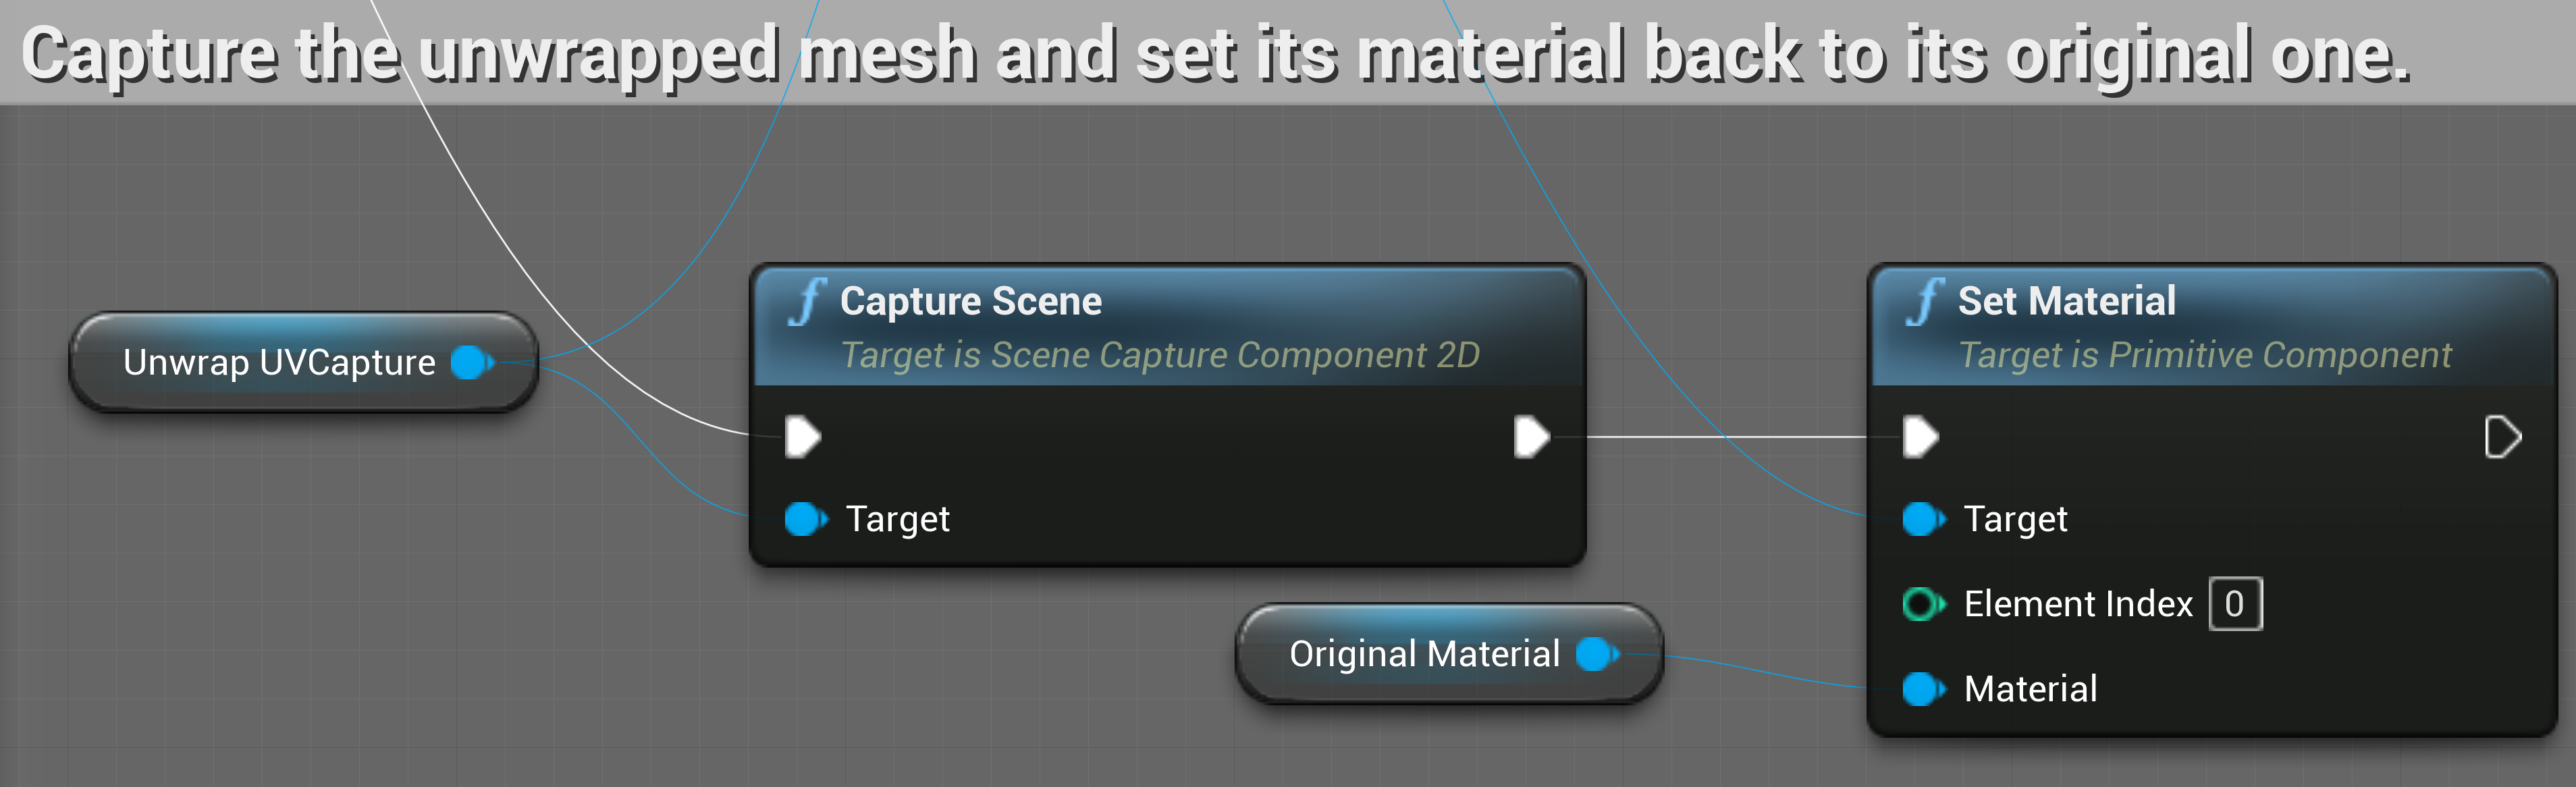
\includegraphics[width=\textwidth]{img/render-splat-2.png}
    \end{subfigure}
    \caption{HeatProducer RenderSplatOntoComponent function.}
    \label{fig:render-splat-function}
\end{figure}

\subsection{GazeEmitter}
\label{sec:gaze-emitter}

It is a~child of the~SceneComponent class and is crucial for the~whole plug-in functionality. It is intended to be added to some user-defined Pawn. After that, the~user can define what they want to use as input to this plug-in. If they wanted to track a~character moving around the~floor of the~scene, all they would need to supply GazeEmitter with is the~position of the~character and a~directional vector to the~ground. This would cause heatmaps to be created on the~floor object, which would be defined as an~EyeTrackedStaticMeshComponent.

At the~beginning of the~game, the~component is constructed and in its \emph{BeginPlay} event, it contains the~spawn node of the~HeatmapProdurer Actor and its assignment to a~private variable, as can be seen in Figure~\ref{fig:emitter-begin}.

\pagebreak{}

\begin{figure}[!ht]
    \centering
    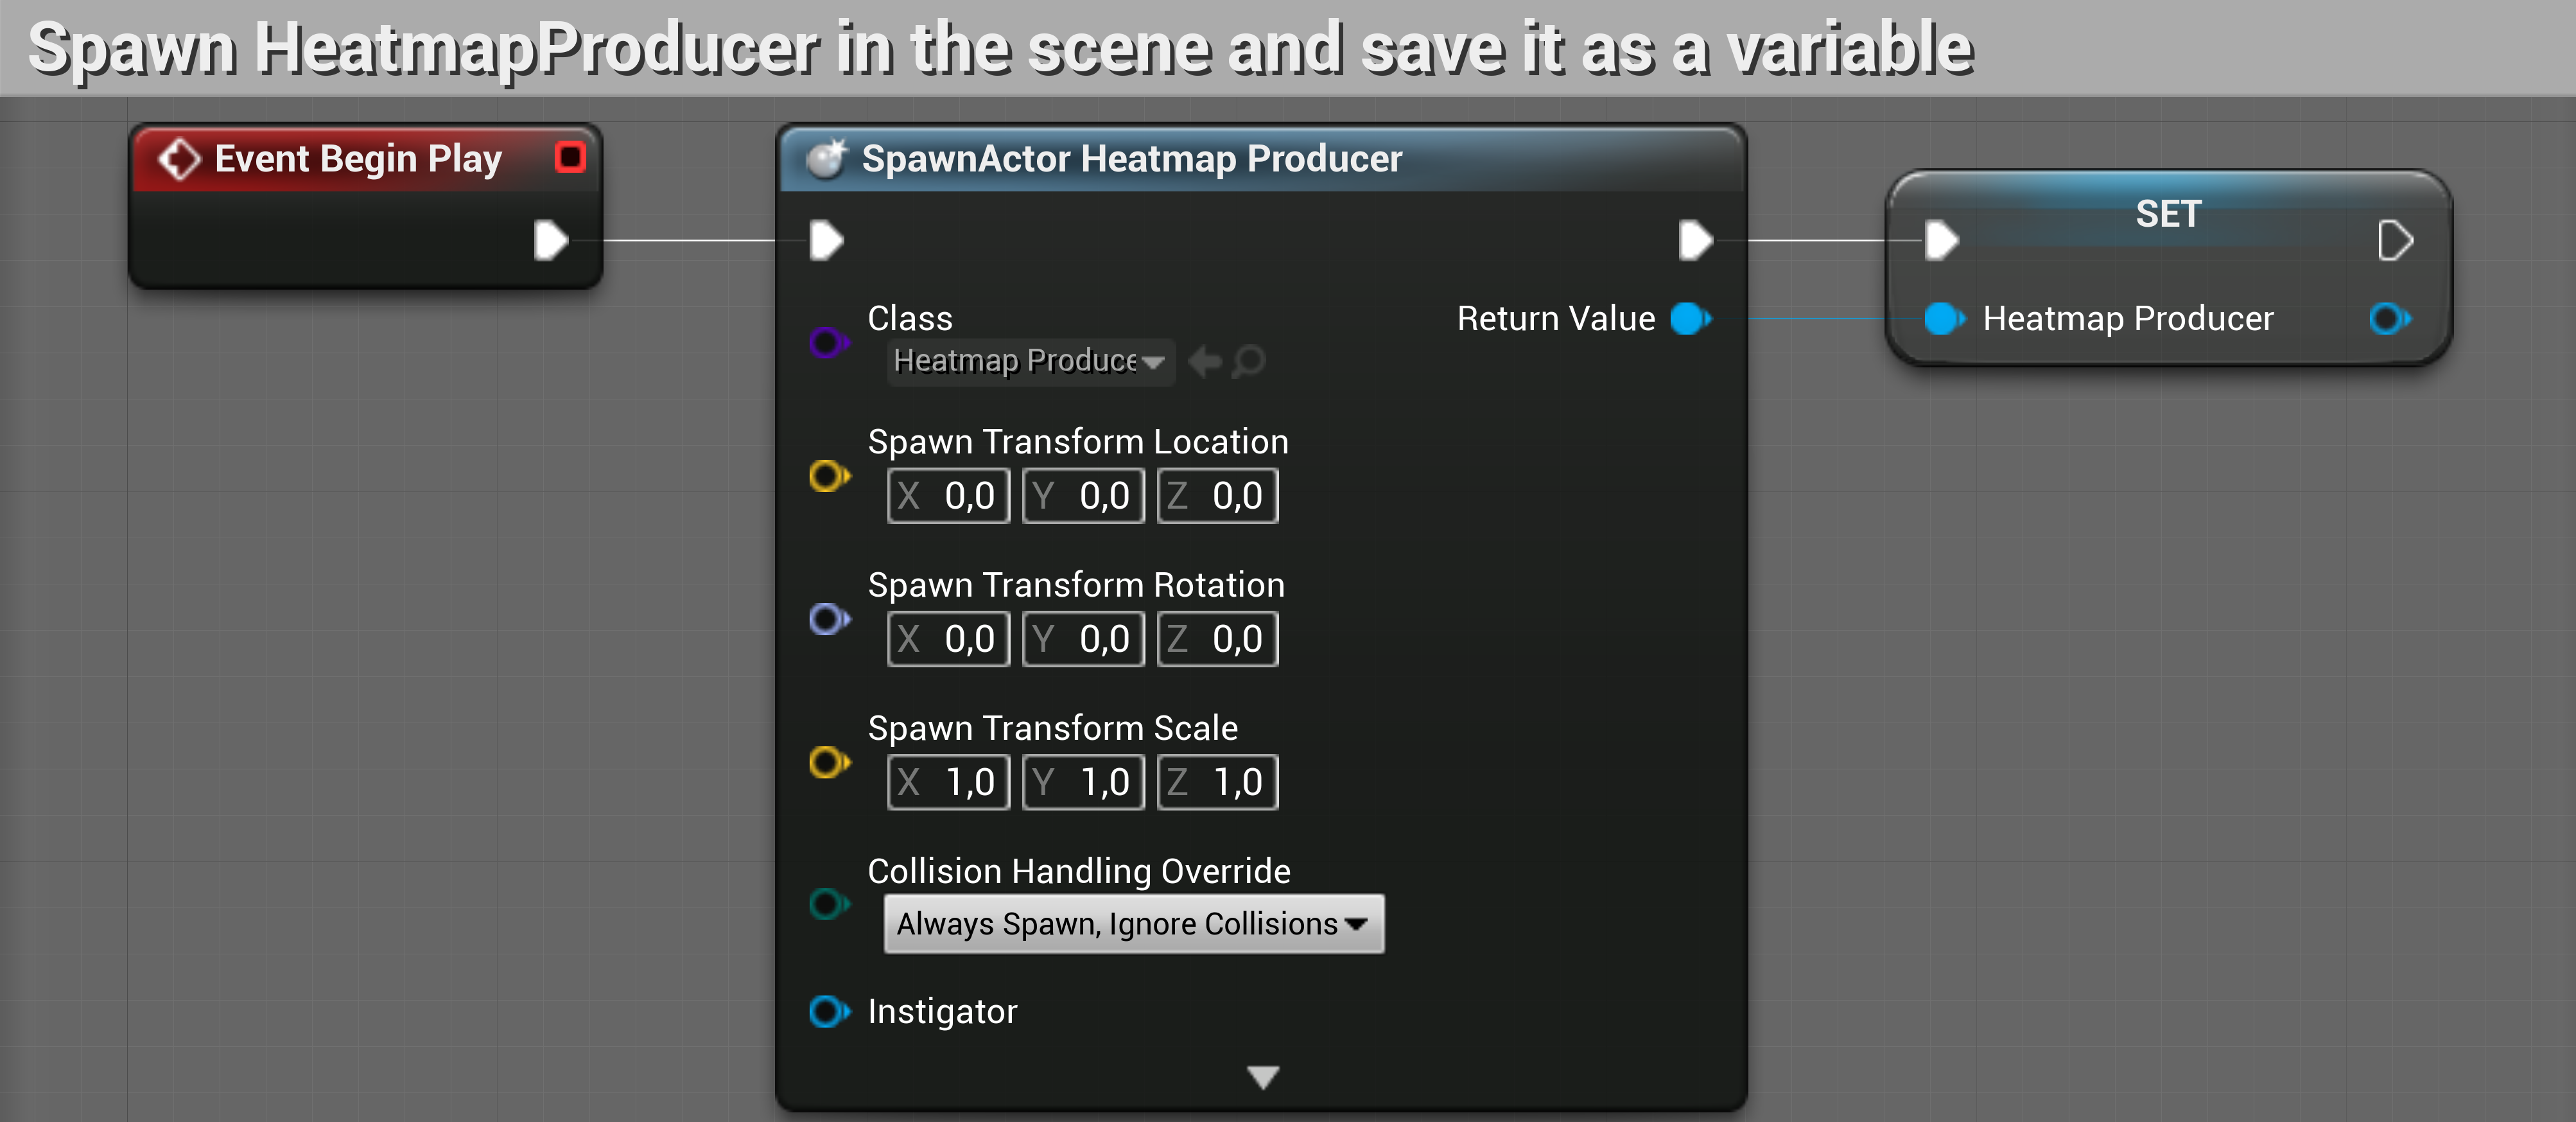
\includegraphics[width=\textwidth]{img/gaze-emitter-begin-play.png}
    \caption{GazeEmitter Event BeginPlay.}
    \label{fig:emitter-begin}
\end{figure}

The~whole functionality consists only of calling \emph{LineTraceForObjects}, which passes the~start and end of a~trace ray that detects a~collision on some object in the~scene. This is done using the~\emph{GetWorldHitFrom} function in Figure~\ref{fig:emitter-world-hit}. If it hits something, it first determines if it is an~EyeTrackedStaticMeshComponent; if so, the~trace was successful.

This first trace was only performed as part of a~simple collision to first know which component is being hit. It cannot be guaranteed that the~simple collision volume will be detailed enough to represent the~entire mesh. If heatmaps were drawn only under these circumstances, it might happen that heat would not be applied to some parts of several objects. Illustrated in the~video with the~path \path{video/03-simple-collision-only.mp4}.

There is a~function in Unreal called \emph{LineTraceComponent} that takes a~component and the~start and end of a~trace ray as input. Its advantage is that it only performs the~tracing on that particular component. Tracing can be set to complex, which will traverse all triangles of a~given mesh to find a~collision. For meshes with a~very high triangle count, this can be a~time consuming operation. 

This is handled by GazeEmitter's \emph{GetComplexFromSimpleHit} function also in Figure~\ref{fig:emitter-world-hit}, which takes a~hit as input, extracts the~trace ray, and sends it again. The~general functionality of creating heatmaps using these functions can be seen in the~\path{video/04-creating-heatmaps.mp4} using a~forward vector of a~virtual camera.

\begin{figure}[!ht]
    \centering
    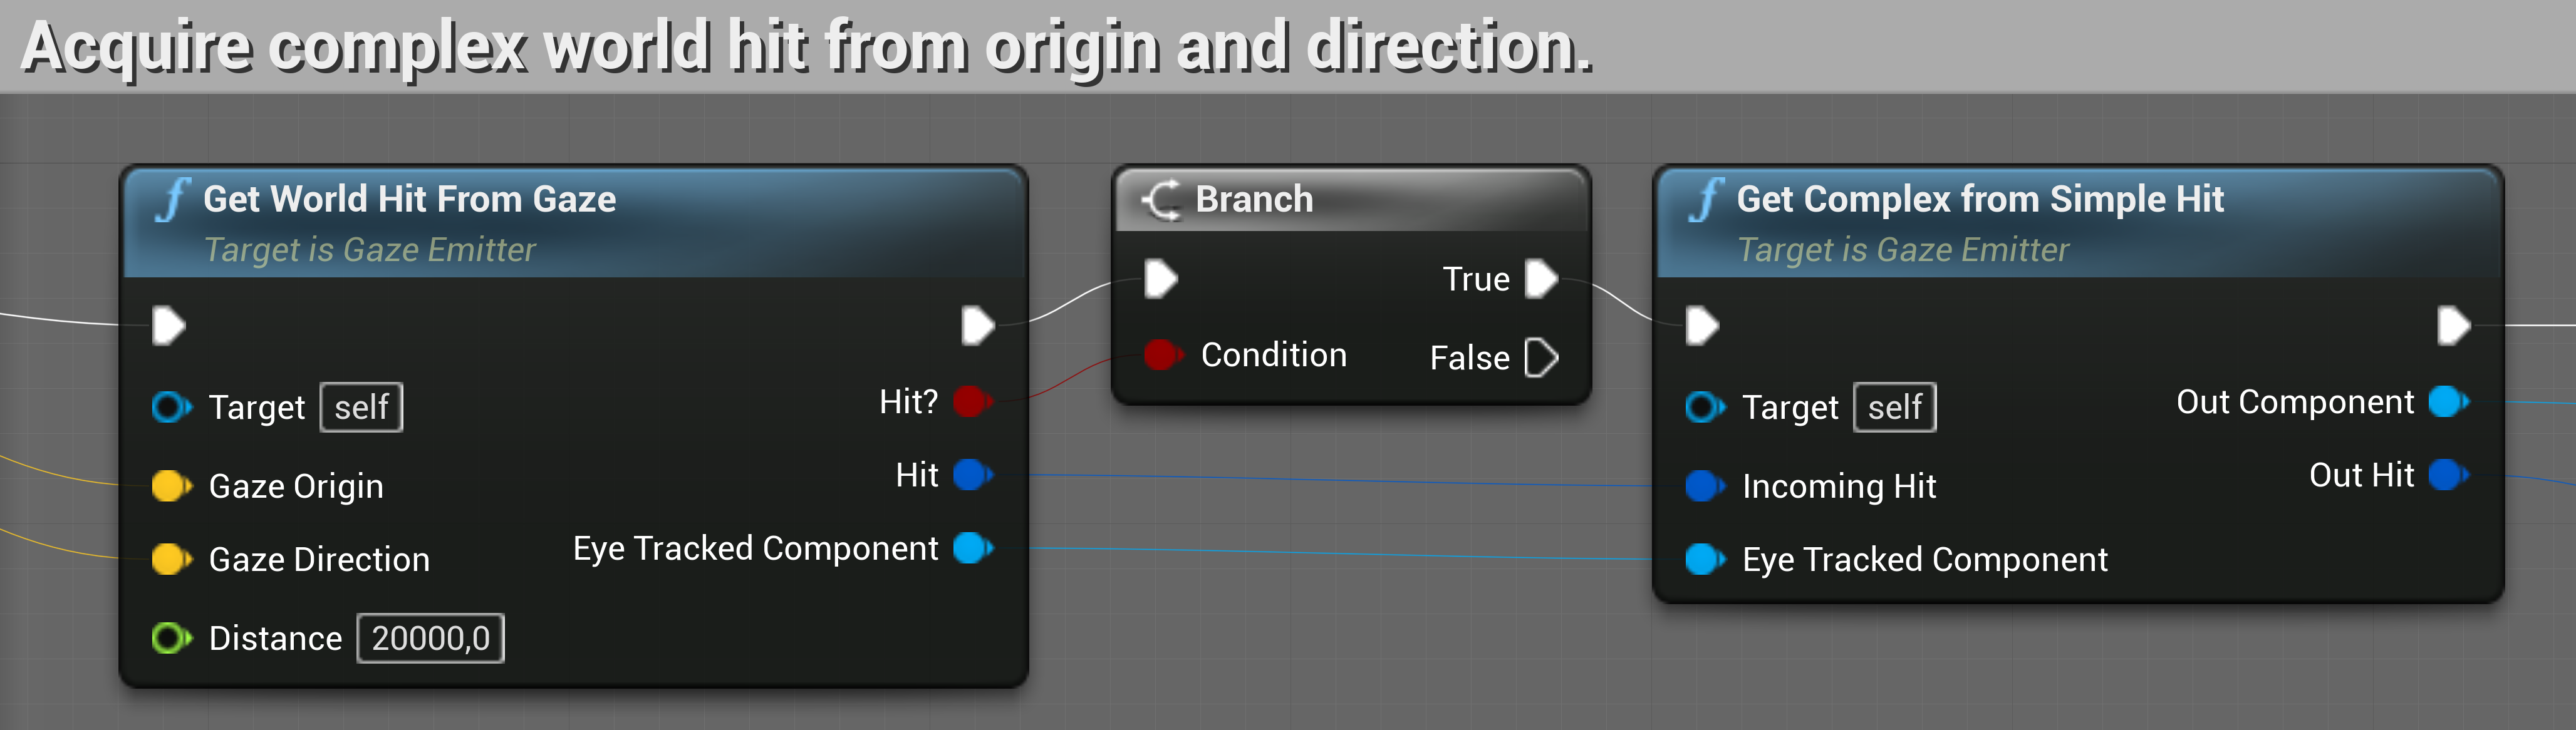
\includegraphics[width=\textwidth]{img/ray-world-hit.png}
    \caption{GazeEmitter get a~complex world hit on a~single component.}
    \label{fig:emitter-world-hit}
\end{figure}

\pagebreak{}

\section{Python}
\label{sec:python}
The~Python section will describe the~script for producing the~resultant data from the~collected EXR textures from different users.

\subsection{EXR image merger script}

This script is used to edit EXR files by iterating through all possible textures of one measurement and one type. This gives a~unique texture for all objects that were part of the~Unreal scene.

\medskip{}
However, these textures exist in multiple variations, depending on how many measurements were made. As a~merging script, it ensures that all these textures are merged into one. This is done simply by dividing all texture values by the~number of variants. These weighted textures are then merged by a~simple add operation.

\medskip{}
For this, the~OpenEXR library~\cite{openexr} is used to perform read and write operations on EXR files, and NumPy~\cite{numpy-doc} to perform these image operations.

\medskip{}
The~OpenXR library always reads the~image channels as strings. Now, it depends on how the~textures are defined. They can be of 32 and 16 bit floats. In the~case of exported textures, they are 16-bit EXR images. Using NumPy, this string is converted just according to \path{numpy.float16}.

\bigskip{}
The~script gets the~paths to all texture files of a~single scene object. Individually reads their red channel as a~string, which is converted to a~numpy array. Creates an~empty 1D 16-bit float buffer of the~size of the~texture's pixel count. Then, it successively loads each red channel of all the~textures into this buffer, multiplied by a~weight constant. The~resultant numpy array is converted back to a~string and exported by the~OpenEXR function, where the~red channel is assigned for both the~green and blue channels. This can be done because the~heatmap trail is a~white image. The~commented source code can be found in the~enclosed media in \path{src/python/merger.py}. 




% \definecolor{codegreen}{rgb}{0,0.6,0}
% \definecolor{codegray}{rgb}{0.5,0.5,0.5}
% \definecolor{codepurple}{rgb}{0.58,0,0.82}
% \definecolor{backcolour}{rgb}{0.95,0.95,0.92}

% \lstdefinestyle{mystyle}{
%     backgroundcolor=\color{backcolour},   
%     commentstyle=\color{codegreen},
%     keywordstyle=\color{magenta},
%     numberstyle=\tiny\color{codegray},
%     stringstyle=\color{codepurple},
%     basicstyle=\ttfamily\footnotesize,
%     breakatwhitespace=false,         
%     breaklines=true,                 
%     captionpos=b,                    
%     keepspaces=true,                 
%     numbers=left,                    
%     numbersep=5pt,                  
%     showspaces=false,                
%     showstringspaces=false,
%     showtabs=false,                  
%     tabsize=2
% }

% \lstset{style=mystyle}

% \lstinputlisting[caption={EXR Heatmap Texture merger script~}, captionpos=b, language=Python]{code/merger.py}
